\chapter{Time series models}\label{chap8}
In this chapter, we provide a brief introduction to performing inference in time series models using a Bayesian framework. There is a large literature in time series in statistics and econometrics, and it would be impossible to present a good treatment in a few pages of an introductory book. However, there are excellent books in Bayesian inference in time series, see for instance, \cite{west2006bayesian,petris2009dynamic,pole2018applied}.

A time series is a sequence of observations collected in chronological order, allowing us to track how variables change over time. However, it also introduces technical challenges, as we must account for statistical features such as autocorrelation and stationarity. Since time series data is time-dependent, we adjust our notation. Specifically, we use $t$ and $T$ instead of $i$ and $N$ to explicitly indicate time.

Our starting point in this chapter is the \textit{state-space representation} of time series models. Much of the Bayesian inference literature in time series adopts this approach, as it allows dynamic systems to be modeled in a structured way. This representation provides modularity, flexibility, efficiency, and interpretability in complex models where the state evolves over time. It also enables the use of recursive estimation methods, such as the \textit{Kalman filter} for dynamic Gaussian linear models and the \textit{particle filter} (also known as \textit{sequential Monte Carlo}) for non-Gaussian and nonlinear state-space models. The latter method is especially useful for \textit{online} predictions or when there are data storage limitations. These inferential tools are based on the sequential updating process of Bayes' rule, where the posterior at time $t$ becomes the prior at time $t+1$ (see Equation \ref{equpdate}).

Remember that we can run our GUI typing

\begin{tcolorbox}[enhanced,width=4.67in,center upper,
	fontupper=\large\bfseries,drop shadow southwest,sharp corners]
	\textit{R code. How to display our graphical user interface}
	\begin{VF}
		\begin{lstlisting}[language=R]
		shiny::runGitHub("besmarter/BSTApp", launch.browser = T)\end{lstlisting}
	\end{VF}
\end{tcolorbox} 

in the \textbf{R} package console or any \textbf{R} code editor, and once our GUI is deployed, select \textit{Time series Models}. However, users should see Chapter \ref{chapGUI} for details.

\section{State-space representation}\label{sec81}
A \textit{state-space model} is composed by of an \textit{unobservable state vector}  $\bm{\beta}_t \in \mathbb{R}^K$, and an \textit{observed} measure $\bm{Y}_t \in \mathbb{R}^M$, $t=1,2,\dots$ such that (i) $\bm{\beta}_t$ is a \textit{Markov process}, this is, $\pi(\bm{\beta}_t\mid \bm{\beta}_{1:t-1})=\pi(\bm{\beta}_t\mid \bm{\beta}_{t-1})$, all the information regarding $\bm{\beta}_t$ based on all its history up to $t-1$ is carried by $\bm{\beta}_{t-1}$, and (ii) $\bm{Y}_t$ is independent of $\bm{Y}_s$ conditional on $\bm{\beta}_t$, $s < t$ \cite[Chap.~2]{petris2009dynamic}.

These assumptions imply that $\pi(\bm{\beta}_{0:t},\bm{Y}_{1:t})=\pi(\bm{\beta}_0)\prod_{s=1}^{t}\pi(\bm{\beta}_s\mid \bm{\beta}_{s-1})\pi(\bm{Y}_s\mid \bm{\beta}_s)$.\footnote{A \textit{state-space model} where the states are random variables taking discrete values is called \textit{hidden Markov model}.}

There are three key aims in \textit{state-space models}: \textit{filtering}, \textit{smoothing}, and \textit{forecasting}. In \textit{filtering}, we aim to estimate the current state given observations up to time $t$, specifically obtaining the density $\pi(\bm{\beta}_{s}\mid \bm{y}_{1:t})$ for $s = t$. In \textit{smoothing}, we conduct a retrospective analysis of the system, obtaining $\pi(\bm{\beta}_{s}\mid \bm{y}_{1:t})$ for $s < t$. In \textit{forecasting}, we forecast future observations by first obtaining $\pi(\bm{\beta}_{s}\mid \bm{y}_{1:t})$ as an intermediate step to compute $\pi(\bm{Y}_{s}\mid \bm{y}_{1:t})$ for $s > t$. A valuable feature of these methods is that all these densities can be calculated recursively. \cite{petris2009dynamic} show the recursive equations in Propositions 2.1 (filtering), 2.3 (smoothing) and 2.5 (forecasting).

An important class of \textit{state-space models} is the \textit{Gaussian linear state-space model}, also know as, \textit{dynamic linear model}:
\begin{align*}
	\bm{Y}_t&=\bm{X}_t\bm{\beta}_t+\bm{\mu}_t& \text{(Observation equations)}\\
	\bm{\beta}_t&=\bm{G}_t\bm{\beta}_{t-1}+\bm{w}_t & \text{(States equations)},
\end{align*}
where $\bm{\beta}_0\sim N(\bm{b}_0,\bm{B}_0)$, $\bm{\mu}_t\sim N(\bm{0}, \bm{\Sigma}_t)$, $\bm{w}_t\sim N(\bm{0}, \bm{\Omega}_t)$, $\bm{\beta}_0$, $\bm{\mu}_t$ and $\bm{w}_t$ are independent, $\bm{X}_t$ and $\bm{G}_t$ are $M\times K$ and $K\times K$ known matrices. Observe that this assumptions implies that $\bm{Y}_t\mid \bm{\beta}_t\sim N(\bm{X}_t\bm{\beta}_t,\bm{\Sigma}_t)$, and $\bm{\beta}_t\mid \bm{\beta}_{t-1}\sim N(\bm{G}_t\bm{\beta}_{t-1},\bm{\Omega}_t)$.\footnote{A general \textit{state-space model} is given by $\bm{Y}_t=\bm{f}_t(\bm{\beta}_t,\bm{\mu}_t)$, and $\bm{\beta}_t=\bm{m}_t(\bm{\beta}_{t-1},\bm{w}_t)$ for arbitrary functions $\bm{f}_t$ and $\bm{m}_t$, and distributions for $\bm{\mu}_t$ and $\bm{w}_t$, and a prior distribution for $\bm{\beta}_0$.}

Let $\bm{\beta}_{t-1}\mid \bm{y}_{1:t-1}\sim N(\bm{b}_{t-1},\bm{B}_{t-1})$, then, we can get the \textit{Kalman filter} by getting
\begin{enumerate}
	\item The one-step-ahead predictive distribution of $\bm{\beta}_t$ given $\bm{y}_{1:t-1}$ is $\bm{\beta}_t\mid \bm{y}_{1:t-1}\sim N(\bm{a}_t, \bm{R}_t)$, where $\bm{a}_t=\bm{G}_t\bm{b}_{t-1}$ and $\bm{R}_t=\bm{G}_t\bm{B}_{t-1}\bm{G}_t^{\top}+\bm{\Omega}_t$.
	\item  The one-step-ahead predictive distribution of $\bm{Y}_t$ given $\bm{y}_{1:t-1}$ is $\bm{Y}_t\mid \bm{y}_{1:t-1}\sim N(\bm{f}_t, \bm{Q}_t)$, where $\bm{f}_t=\bm{X}_t\bm{a}_t$ and $\bm{Q}_t=\bm{X}_t\bm{R}_t\bm{X}_t^{\top}+\bm{\Sigma}_t$.
	\item The distribution of the one-step-ahead prediction error  $\bm{e}_t=\bm{Y}_t-\mathbb{E}[\bm{Y}_t\mid \bm{y}_{1:t-1}]=\bm{Y}_t-\bm{f}_t$ is $N(\bm{0}, \bm{Q}_t)$ \cite[Chap.~6]{shumway2017time}. 
	\item The filtering distribution of $\bm{\beta}_t$ given $\bm{y}_{1:t}$ is $\bm{\beta}_t\mid \bm{y}_{1:t}\sim N(\bm{b}_t, \bm{B}_t)$, where $\bm{b}_t=\bm{a}_t+\bm{K}_t\bm{e}_t$, $\bm{K}_t=\bm{R}_t\bm{X}_t^{\top}\bm{Q}_t^{-1}$ is the \textit{Kalman gain}, and $\bm{B}_t=\bm{R}_t-\bm{R}_t\bm{X}_t^{\top}\bm{Q}_t^{-1}\bm{X}_t\bm{R}_t$.   
\end{enumerate}    

The formal proofs of these results can be found in \cite[Chap~2]{petris2009dynamic}. Just take into account that the logic of these results follow the results of the Seemingly unrelated regression (SUR) model in Section \ref{sec72} for a particular time period. In addition, we know that the posterior distribution using information up to $t-1$ becomes the prior in $t$ (see Equation \ref{equpdate}, $\pi(\bm{\theta}\mid \mathbf{y}_{1:t})\propto p(y_{t}\mid \bm{y}_{1:t-1},\bm{\theta})\times \pi(\bm{\theta}\mid \bm{y}_{1:t-1})$). This is the updating process from  $\bm{\beta}_t\mid \bm{y}_{1:t-1}\sim N(\bm{a}_t, \bm{R}_t)$ to $\bm{\beta}_t\mid \bm{y}_{1:t}\sim N(\bm{b}_t, \bm{B}_t)$. Moreover, the posterior mean and variance of the SUR model with independent conjugate priors for a particular time period can be written as $\bm{a}_{t}+\bm{R}_{t}\bm{X}_t^{\top}(\bm{X}_t\bm{R}_{t}\bm{X}_t^{\top}+ \bm{\Sigma}_t)^{-1}(\bm{y}_t-\bm{X}_t\bm{a}_{t})$ and $\bm{R}_{t}-\bm{R}_{t}\bm{X}_t^{\top}(\bm{X}_t\bm{R}_{t}\bm{X}_t^{\top}+\bm{\Sigma}_t)^{-1} \bm{X}_t\bm{R}_{t}^{\top}$, respectively. Let's see this, we know from Section \ref{sec72} that $\bm{B}_t=(\bm{R}_t^{-1}+\bm{X}_t^{\top}\bm{\Sigma}^{-1}\bm{X}_t)^{-1}$ and $\bm{\beta}_t=\bm{B}_t(\bm{R}_t^{-1}\bm{a}_t+\bm{X}_t^{\top}\bm{\Sigma}^{-1}\bm{y}_t)$. Thus, let's show that both conditional posterior distributions are the same. In particular, the posterior mean in the \textit{state-space representation} is $[\bm{I}_K-\bm{R}_{t}\bm{X}_t^{\top}(\bm{X}_t\bm{R}_{t}\bm{X}_t^{\top}+ \bm{\Sigma}_t)^{-1}\bm{X}_t]\bm{a}_{t}+\bm{R}_{t}\bm{X}_t^{\top}(\bm{X}_t\bm{R}_{t}\bm{X}_t^{\top}+ \bm{\Sigma}_t)^{-1}\bm{y}_t$, where 
\begin{align*}
	\bm{R}_{t}\bm{X}_t^{\top}(\bm{X}_t\bm{R}_{t}\bm{X}_t^{\top}+ \bm{\Sigma}_t)^{-1}
	&=\bm{R}_{t}\bm{X}_t^{\top}[\bm{\Sigma}_t^{-1}-\bm{\Sigma}_t^{-1}\bm{X}_t(\bm{R}_t^{-1}+\bm{X}_t^{\top}\bm{\Sigma}_t^{-1}\bm{X}_t)^{-1}\bm{X}_t^{\top}\bm{\Sigma}_t^{-1}]\\
	&=\bm{R}_{t}[\bm{I}_K-\bm{X}_t^{\top}\bm{\Sigma}_t^{-1}\bm{X}_t(\bm{R}_t^{-1}+\bm{X}_t^{\top}\bm{\Sigma}_t^{-1}\bm{X}_t)^{-1}]\bm{X}_t^{\top}\bm{\Sigma}_t^{-1}\\
	&=\bm{R}_{t}(\bm{I}_K-[\bm{I}_K-\bm{R}_t^{-1}(\bm{R}_t^{-1}+\bm{X}_t^{\top}\bm{\Sigma}_t^{-1}\bm{X}_t)^{-1}])\bm{X}_t^{\top}\bm{\Sigma}_t^{-1}\\
	&=(\bm{R}_t^{-1}+\bm{X}_t^{\top}\bm{\Sigma}_t^{-1}\bm{X}_t)^{-1}\bm{X}_t^{\top}\bm{\Sigma}_t^{-1},
\end{align*}
where the first equality uses the Woodbury matrix identity (matrix inversion lemma), and the third equality uses $\bm{D}(\bm{D}+\bm{E})^{-1}=\bm{I}-\bm{E}(\bm{D}+\bm{E})^{-1}$.

Thus, we have the following expression:
\begin{flalign*}
	&[\bm{I}_K - \bm{R}_t \bm{X}_t^{\top} (\bm{X}_t \bm{R}_t \bm{X}_t^{\top} + \bm{\Sigma}_t)^{-1} \bm{X}_t] \bm{a}_t + \bm{R}_t \bm{X}_t^{\top} (\bm{X}_t \bm{R}_t \bm{X}_t^{\top} + \bm{\Sigma}_t)^{-1} \bm{y}_t \\
	&= [\bm{I}_K - (\bm{R}_t^{-1} + \bm{X}_t^{\top} \bm{\Sigma}_t^{-1} \bm{X}_t)^{-1} \bm{X}_t^{\top} \bm{\Sigma}_t^{-1} \bm{X}_t] \bm{a}_t + (\bm{R}_t^{-1} + \bm{X}_t^{\top} \bm{\Sigma}_t^{-1} \bm{X}_t)^{-1} \bm{X}_t^{\top} \bm{\Sigma}_t^{-1} \bm{y}_t \\
	&= (\bm{R}_t^{-1} + \bm{X}_t^{\top} \bm{\Sigma}_t^{-1} \bm{X}_t)^{-1} \bm{R}_t^{-1} \bm{a}_t + (\bm{R}_t^{-1} + \bm{X}_t^{\top} \bm{\Sigma}_t^{-1} \bm{X}_t)^{-1} \bm{X}_t^{\top} \bm{\Sigma}_t^{-1} \bm{y}_t \\
	&= (\bm{R}_t^{-1} + \bm{X}_t^{\top} \bm{\Sigma}_t^{-1} \bm{X}_t)^{-1} (\bm{R}_t^{-1} \bm{a}_t + \bm{X}_t^{\top} \bm{\Sigma}_t^{-1} \bm{y}_t) \\
	&= (\bm{R}_t^{-1} + \bm{X}_t^{\top} \bm{\Sigma}_t^{-1} \bm{X}_t)^{-1} (\bm{R}_t^{-1} \bm{a}_t + \bm{X}_t^{\top} \bm{\Sigma}_t^{-1} \bm{X}_t \hat{\bm{\beta}}_t),
\end{flalign*}

where the second equality uses the identity:

\[
\bm{I} - (\bm{D} + \bm{E})^{-1} \bm{D} = (\bm{D} + \bm{E})^{-1} \bm{E},
\]

and the estimator \(\hat{\bm{\beta}}_t\) is defined as:

\[
\hat{\bm{\beta}}_t = (\bm{X}_t^{\top} \bm{\Sigma}_t^{-1} \bm{X}_t)^{-1} \bm{X}_t^{\top} \bm{\Sigma}_t^{-1} \bm{y}_t.
\]

This shows that the posterior mean is a weighted average of the prior mean and the maximum likelihood estimator (which is the generalized least squares estimator).
 
The weights are linked to the signal-to-noise ratio, that is, the proportion of the total variability ($\bm{\Omega}_t+\bm{\Sigma}_t$) due to the signal ($\bm{\Omega}_t$) versus the noise ($\bm{\Sigma}_t$). Note that in the simplest case where $M=K=1$, and $\bm{X}_t=\bm{G}_t=1$, then $\bm{K}_t=\bm{R}_t\bm{Q}_t^{-1}=(B_{t-1}+\Omega_t)/(B_{t-1}+\Omega_t+\Sigma_t)$. Thus, the weight associated with the observations is equal to 1 if $\Sigma_t=0$, that is, the posterior mean is equal to the actual observation. On the other hand, if $\Sigma_t$ increases compare to $\Omega_t$, there is more weight to the prior information, and consequently, the posterior mean is smoother as it heavily dependents on the history. We ask in Exercise 1 to perform simulations with different signal-to-noise ratios to see the effects on the system.   

The equality of variances of both approaches is as follows:
\begin{align*}
	Var[\bm{\beta}_t\mid \bm{y}_{1:t}]&
	= \bm{R}_{t}-\bm{R}_{t}\bm{X}_t^{\top}(\bm{X}_t\bm{R}_{t}\bm{X}_t^\top+\bm{\Sigma}_t)^{-1} \bm{X}_t\bm{R}_{t}\\
	&=\bm{R}_{t}-\bm{R}_{t}\bm{X}_t^{\top}(\bm{\Sigma}_t^{-1}- \bm{\Sigma}_t^{-1}\bm{X}_t(\bm{R}_{t}^{-1}+\bm{X}_t^{\top}\bm{\Sigma}_t^{-1}\bm{X}_t)^{-1}\bm{X}_t^{\top}\bm{\Sigma}_t^{-1})\bm{X}_t\bm{R}_{t}\\
	&=\bm{R}_{t}-\bm{R}_{t}\bm{X}_t^{\top}\bm{\Sigma}_t^{-1}\bm{X}_t\bm{R}_{t}+ \bm{R}_{t}\bm{X}_t^{\top}\bm{\Sigma}_t^{-1}\bm{X}_t(\bm{R}_{t}^{-1}+\bm{X}_t^{\top}\bm{\Sigma}_t^{-1}\bm{X}_t)^{-1}\bm{X}_t^{\top}\bm{\Sigma}_t^{-1}\bm{X}_t\bm{R}_{t}\\
	&=\bm{R}_{t}-\bm{R}_{t}\bm{X}_t^{\top}\bm{\Sigma}_t^{-1}\bm{X}_t\bm{R}_{t}+ \bm{R}_{t}\bm{X}_t^{\top}\bm{\Sigma}_t^{-1}\bm{X}_t[\bm{I}_K-(\bm{R}_{t}^{-1}+\bm{X}_t^{\top}\bm{\Sigma}_t^{-1}\bm{X}_t)^{-1}\bm{R}_{t}^{-1}]\bm{R}_{t}\\
	&=\bm{R}_{t}-\bm{R}_{t}\bm{X}_t^{\top}\bm{\Sigma}_t^{-1}\bm{X}_t(\bm{R}_{t}^{-1}+\bm{X}_t^{\top}\bm{\Sigma}_t^{-1}\bm{X}_t)^{-1}\\
	&=\bm{R}_t[\bm{I}_K-\bm{X}_t^{\top}\bm{\Sigma}_t^{-1}\bm{X}_t(\bm{R}_{t}^{-1}+\bm{X}_t^{\top}\bm{\Sigma}_t^{-1}\bm{X}_t)^{-1}]\\
	&=\bm{R}_{t}[\bm{I}_K-(\bm{I}_K-\bm{R}_{t}^{-1}(\bm{R}_{t}^{-1}+\bm{X}_t^{\top}\bm{\Sigma}_t^{-1}\bm{X}_t)^{-1})]\\
	&=(\bm{R}_{t}^{-1}+\bm{X}_t^{\top}\bm{\Sigma}_t^{-1}\bm{X}_t)^{-1},
\end{align*}
where the second equality uses the Woodbury matrix identity, the fourth equality uses $(\bm{D}+\bm{E})^{-1}\bm{D}=\bm{I}-(\bm{D}+\bm{E})^{-1}\bm{E}$, and the seventh equality uses $\bm{D}(\bm{D}+\bm{E})^{-1}=\bm{I}-\bm{E}(\bm{D}+\bm{E})^{-1}$.  

The \textit{Kalman filter} allows calculating recursively in a forward way $\pi(\bm{\beta}_t\mid \bm{y}_{1:t})$ from $\pi(\bm{\beta}_{t-1}\mid \bm{y}_{1:t-1})$ starting from $\pi(\bm{\beta}_0)$.

Let $\bm{\beta}_{t+1}\mid \bm{y}_{1:T}\sim N(\bm{s}_{t+1},\bm{S}_{t+1})$, then we can get the \textit{Kalman smoother} by $\bm{\beta}_{t}\mid \bm{y}_{1:T}\sim N(\bm{s}_{t},\bm{S}_{t})$, where $\bm{s}_t=\bm{b}_t+\bm{B}_t\bm{G}_{t+1}^{\top}\bm{R}_{t+1}^{-1}(\bm{s}_{t+1}-\bm{a}_{t+1})$ and $\bm{S}_t=\bm{B}_t-\bm{B}_t\bm{G}_{t+1}^{\top}\bm{R}_{t+1}^{-1}(\bm{R}_{t+1}-\bm{S}_{t+1})\bm{R}_{t+1}^{-1}\bm{G}_{t+1}\bm{B}_{t}$. The proof can be found in \cite[Chap~2]{petris2009dynamic}. 

Thus, we can calculate the \textit{Kalman smoother} starting from $t=T-1$, that is, $\bm{\beta}_{T}\mid \bm{y}_{1:T}\sim N(\bm{s}_{T},\bm{S}_{T})$. However, this is the filtering distribution at $T$, which means $\bm{s}_{T}=\bm{b}_{T}$ and $\bm{S}_{T}=\bm{B}_{T}$, and then, we should proceed recursively in a backward way.

Finally, the forecasting recursion in the \textit{dynamic linear model}, given $\bm{a}_t(0)=\bm{b}_t$ and $\bm{R}_t(0)=\bm{B}_t$, $h\geq 1$, is given by 
\begin{enumerate}
	\item The forecasting distribution of $\bm{\beta}_{t+h}\mid \bm{y}_{1:t}$ is $N(\bm{a}_t(h),\bm{R}_t(h))$, where $\bm{a}_t(h)=\bm{G}_{t+h}\bm{a}_{t}(h-1)$ and $\bm{R}_t(h)=\bm{G}_{t+h}\bm{R}_t(h-1)\bm{G}_{t+h}^{\top}+\bm{\Omega}_{t+h}$.
	\item The forecasting distribution $\bm{Y}_{t+h}\mid \bm{y}_{1:t}$ is $N(\bm{f}_t(h),\bm{Q}_t(h))$, where $\bm{f}_t(h)=\bm{X}_{t+h}\bm{a}_t(h)$ and $\bm{Q}_t(h)=\bm{X}_{t+h}\bm{R}_t(h)\bm{X}_{t+h}^{\top}+\bm{\Sigma}_{t+h}$.  
\end{enumerate}
The proof can be found in \cite[Chap~2]{petris2009dynamic}.

These recursive equations allow us to perform probabilistic forecasting $h$-steps-ahead for the state and observation equations.

These results demonstrate how to use these recursive equations for filtering, smoothing, and forecasting in \textit{dynamic linear models} (\textit{Gaussian linear state-space models}). Although these algorithms appear simple, they suffer from numerical instability, which can lead to non-symmetric and negative-definite covariance matrices. Thus, special care must be taken when working with them.

In addition, this setup assumes that $\bm{\Sigma}_t$ and $\bm{\Omega}_t$ are known. However, this is rarely the case in most situations. Therefore, we need to estimate them. One option is to perform maximum likelihood estimation. However, this approach does not account for the uncertainty associated with the fact that $\bm{\Sigma}_t$ and $\bm{\Omega}_t$ are unknown when their estimates are \textit{plugged into} the \textit{state space} recursions. On the other hand, we can use a Bayesian approach and perform the recursions associated with each posterior draw of the unknown parameters, thus taking their uncertainty into account.

The point of departure is the posterior distribution, such that
\begin{align*}
	\pi(\bm{\theta},\bm{\beta}_0,\dots,\bm{\beta}_T\mid \bm{y}, \bm{X}, \bm{G})&\propto\pi(\bm{\beta}_0\mid \bm{\theta})\pi(\bm{\theta})\prod_{t=1}^{T}\pi(\bm{\beta}_t\mid \bm{\beta}_{t-1},\bm{\theta})\pi(\bm{y}_t\mid \bm{\beta}_t,\bm{\theta}),
\end{align*} 
where $\bm{\theta}$ is the vector of unknown parameters.

We can compute $\pi(\bm{\beta}_s,\bm{\theta}\mid \bm{y}_{1:t})=\pi(\bm{\beta}_s\mid \bm{y}_{1:t},\bm{\theta})\pi(\bm{\theta}\mid \bm{y}_{1:t})$, for $s=t$ (\textit{filtering}), $s<t$ (\textit{smoothing}), and $s>t$ (\textit{forecasting}). The marginal posterior distribution of the states is $\pi(\bm{\beta}_s\mid \bm{y}_{1:t})=\int_{\bm{\Theta}}\pi(\bm{\beta}_s\mid \bm{y}_{1:t},\bm{\theta})\pi(\bm{\theta}\mid \bm{y}_{1:t})d\bm{\theta}$.

We can use the Gibbs sampling algorithm to get the posterior draws in the \textit{dynamic linear model} assuming conjugate families. In particular, let's see the univariate case with \textit{random walk states}, 
\begin{align}
	y_t&=\bm{x}_t^{\top}\bm{\beta}_t+\mu_t\label{eq1Obs}\\
	\bm{\beta}_t&=\bm{\beta}_{t-1}+\bm{w}_t \label{eq1St},
\end{align}
where $\mu_t\sim N(0,\sigma^2)$ and $\bm{w}_t\sim N(\bm{0},\text{diag}\left\{\omega_1^2,\dots,\omega_K^2\right\})$. We assume that $\pi(\sigma^2,\omega_1^2,\dots,\omega_K^2,\bm{\beta}_0)=\pi(\sigma^2)\pi(\omega_1^2),\dots,\pi(\omega_K^2)\pi(\bm{\beta}_0)$ where $\sigma^2\sim IG(\alpha_0/2,\delta_0/2)$, $\omega_k^2\sim IG(\alpha_{k0}/2,\delta_{k0}/2)$, $k=1,\dots,K$, and $\bm{\beta}_0\sim N(\bm{b}_0,\bm{B}_0)$. Thus, the conditional posterior distributions are $\sigma^2\mid \bm{y},\bm{X},\bm{\beta}_{1:T}\sim IG(\alpha_{n}/2,\delta_n/2)$, where $\alpha_{n}=T+\alpha_0$ and $\delta_n=\sum_{t=1}^T(y_t-\bm{x}_t^{\top}\bm{\beta}_t)^2+\delta_0$, and $\omega_k^2\mid \bm{y},\bm{X},\bm{\beta}_{0:T}\sim IG(\alpha_{kn}/2,\delta_{kn}/2)$, where $\alpha_{kn}=T+\alpha_{k0}$ and $\delta_{kn}=\sum_{t=1}^T(\bm{\beta}_{t,k}-\bm{\beta}_{t-1,k})^2+\delta_{k0}$. The vector of the dependent variable is $\bm{y}$, and all regressors are in $\bm{X}$.

We also need to sample the states from $\pi(\bm{\beta}_{1:T}\mid \bm{y},\bm{X},\sigma^2,\omega_1^2,\dots,\omega_K^2)$. This can be done using the \textit{forward filtering backward sampling} (FFBS) algorithm \cite{carter1994gibbs,fruhwirth1994data,shephard1994partial}. This algorithm is basically a simulation version of the \textit{smoothing} recursion, which allows getting draws of the states, even if we do not have analytical solutions, for instance, in non-linear settings. See below and \cite[Chap.~3]{petris2009dynamic} for details. A word of caution here, users should be careful to set non-informative priors in this setting, and in general, settings where there are a large number of parameters (see \cite[Chap.~8]{koop2003bayesian} for details). Thus, it is useful to use empirical Bayes methods focusing on relevant hyperparameters, for instance, the hyperparameters of the inverse-gamma distributions which define the signal-to-noise ratio.   

We use the command \textit{dlmGibbsDIG} from the \textit{dlm} package in our GUI to perform Bayesian inference in the univariate \textit{dynamic linear model} with \textit{random walk states}. This function uses the FFBS algorithm, and assumes independent gamma priors for the precision (inverse of variance) parameters. In addition, this package uses the singular value decomposition to calculate the covariance matrices to avoid numerical instability.

Algorithm \ref{alg:DLM} shows how to perform inference in the univariate \textit{dynamic linear model} with random walk states in our GUI. See also Chapter \ref{chapGUI} for details regarding the dataset structure.

\begin{algorithm}[h!]
	\caption{Dynamic linear models}\label{alg:DLM}
	\begin{algorithmic}[1]  		 			
		\State Select \textit{Time series Model} on the top panel
		\State Select \textit{Dynamic linear model} using the left radio button
		\State Upload the dataset selecting first if there is header in the file, and the kind of separator in the \textit{csv} file of the dataset (comma, semicolon, or tab). Then, use the \textit{Browse} button under the \textbf{Choose File} legend
		\State Select MCMC iterations, burn-in and thinning parameters using the \textit{Range sliders}
		%\State Set the hyperparameters of the \textit{initial states}: prior mean and variance. This step is not necessary as by default our GUI uses non-informative priors.
		\State Set the hyperparameters of the \textit{precision of the observation equation}: prior mean and variance.
		\State Set the hyperparameters of the \textit{pricision of the state equations}: just one set of prior mean and variance parameters.
		\State Click the \textit{Go!} button
		\State Analyze results
		\State Download posterior chains of variances of observation and state equations, and posterior chains of states using the \textit{Download Results} button
	\end{algorithmic} 
\end{algorithm}

\textbf{Example: Simulation exercise of the dynamic linear model}

We simulate the process $y_t=\beta_{t1}+{x}_t{\beta}_{t2}+\mu_t$ and $\bm{\beta}_t=\bm{\beta}_{t-1}+\bm{w}_t$, $t=1,2,\dots,200$, where $\bm{\beta}_t=[\beta_{t1} \ {\beta}_{t2}]^{\top}$, $\mu_t\sim N(0,0.5^2)$, $\bm{w}_t\sim N(\bm{0},\text{diag}\left\{0.2,0.1\right\})$, $x_t\sim N(1, 1)$, $\bm{\beta}_0$ and $\bm{B}_0$ are the OLS estimates and variance of the recursive OLS estimates (see below), respectively.

The following algorithm demonstrates how to perform inference using \textit{dlmGibbsDIG} and compares the results to those of the maximum likelihood estimator, which is based on the \textit{dlmMLE} function. We also use the \textit{dlmSvd2var} function, which is based on singular value decomposition, to calculate the variance of the smoothing states. All these functions are from the \textit{dlm} package in \textbf{R}.

Users can observe that we employ a straightforward strategy for setting the hyperparameters. First, we recursively estimate the model using ordinary least squares (OLS), progressively increasing the sample size, and save the location parameters. Next, we compute the covariance matrix of this sequence and use it to set the priors: the prior mean of the precision of the state vector is set equal to the inverse of the maximum element of the main diagonal of this covariance matrix (\textit{a.theta}), and the prior variance is set equal to ten times this value (\textit{b.theta}). For the observation equation, the prior mean of the precision is set equal to the inverse of the OLS variance estimate (\textit{a.y}), and the prior variance is set equal to ten times this value (\textit{b.y}). We perform some sensitivity analysis of the results regarding the hyperparameters, and it seems that the results are robust. However, we encourage giving more consideration to empirical Bayes methods for setting hyperparameters in \textit{state-space models}.

\begin{tcolorbox}[enhanced,width=4.67in,center upper,
	fontupper=\large\bfseries,drop shadow southwest,sharp corners]
	\textit{R code. Simulation: Dynamic linear model}
	\begin{VF}
		\begin{lstlisting}[language=R]
rm(list = ls()); set.seed(010101)
T <- 200; sig2 <- 0.5^2
x <- rnorm(T, mean = 1, sd = 1) 
X <- cbind(1, x); B0 <- c(1, 0.5)
K <- length(B0)
e <- rnorm(T, mean = 0, sd = sig2^0.5)
Omega <- diag(c(0.2, 0.1))
w <- MASS::mvrnorm(T, c(0, 0), Omega)
Bt <- matrix(NA, T, K); Bt[1,] <- B0
yt <- rep(NA, T) 
yt[1] <- X[1,]%*%B0 + e[1]
for(t in 1:T){
	if(t == 1){
		Bt[t,] <- w[t,]
	}else{
		Bt[t,] <- Bt[t-1,] + w[t,]
	}
	yt[t] <- X[t,]%*%Bt[t,] + e[t]
}
RegLS <- lm(yt ~ x)
SumRegLS <- summary(RegLS)
SumRegLS; SumRegLS$sigma^2  
Bp <- matrix(RegLS$coefficients, T, K, byrow = TRUE)
S <- 20
for(t in S:T){
	RegLSt <- lm(yt[1:t] ~ x[1:t])
	Bp[t,] <- RegLSt$coefficients 
}
# plot(Bp[S:T,2], type = "l")
VarBp <- var(Bp)
# State space model
ModelReg <- function(par){
	Mod <- dlm::dlmModReg(x, dV = exp(par[1]), dW = exp(par[2:3]), m0 = RegLS$coefficients,	C0 = VarBp)
	return(Mod)
}
outMLEReg <- dlm::dlmMLE(yt, parm = rep(0, K+1), ModelReg)
exp(outMLEReg$par)
RegFilter <- dlm::dlmFilter(yt, ModelReg(outMLEReg$par))
RegSmoth <- dlm::dlmSmooth(yt, ModelReg(outMLEReg$par))
SmoothB2 <- RegSmoth$s[-1,2]
VarSmooth <- dlm::dlmSvd2var(u = RegSmoth[["U.S"]], RegSmoth[["D.S"]])
SDVarSmoothB2 <- sapply(2:(T+1), function(t){VarSmooth[[t]][K,K]^0.5}) 
LimInfB2 <- SmoothB2 - qnorm(0.975)*SDVarSmoothB2
LimSupB2 <- SmoothB2 + qnorm(0.975)*SDVarSmoothB2
# Gibbs
MCMC <- 2000; burnin <- 1000
a.y <- (SumRegLS$sigma^2)^(-1); b.y <- 10*a.y; a.theta <- (max(diag(VarBp)))^(-1); b.theta <- 10*a.theta 
gibbsOut <- dlm::dlmGibbsDIG(yt, mod = dlm::dlmModReg(x), a.y = a.y, b.y = b.y, a.theta = a.theta, b.theta = b.theta, n.sample = MCMC, thin = 5, save.states = TRUE)
\end{lstlisting}
	\end{VF}
\end{tcolorbox} 
 
\begin{tcolorbox}[enhanced,width=4.67in,center upper,
	fontupper=\large\bfseries,drop shadow southwest,sharp corners]
	\textit{R code. Simulation: Dynamic linear model}
	\begin{VF}
		\begin{lstlisting}[language=R]
B2t <- matrix(0, MCMC - burnin, T + 1)
for(t in 1:(T+1)){
	B2t[,t] <- gibbsOut[["theta"]][t,2,-c(1:burnin)] 
}
Lims <- apply(B2t, 2, function(x){quantile(x, c(0.025, 0.975))})
summary(coda::mcmc(gibbsOut[["dV"]]))
summary(coda::mcmc(gibbsOut[["dW"]]))
# Figure
require(latex2exp) # LaTeX equations in figures
xx <- c(1:(T+1), (T+1):1)
yy <- c(Lims[1,], rev(Lims[2,]))
plot   (xx, yy, type = "n", xlab = "Time", ylab = TeX("$\\beta_{t2}$"))
polygon(xx, yy, col = "lightblue", border = "lightblue")
xxML <- c(1:T, T:1)
yyML <- c(LimInfB2, rev(LimSupB2))
polygon(xxML, yyML, col = "blue", border = "blue")
lines(colMeans(B2t), col = "red", lw = 2)
lines(Bt[,2], col = "black", lw = 2)
lines(SmoothB2, col = "green", lw = 2)
title("State vector: Slope parameter")
\end{lstlisting}
	\end{VF}
\end{tcolorbox}

Figure \ref{fig1} shows the comparison between maximum likelihood (ML) and Bayesian inference. The light blue (Bayesian) and dark blue (maximum likelihood) shadows show the credible and confidence intervals at 95\% for the state slope parameter ($\beta_{t2}$). We see that the Bayesian interval encompass the ML interval. This is a reflection of the extra uncertainty of the unknown variances. The black line is the actual trajectory of $\beta_{t2}$, the green and red lines are the \textit{smoothing} recursions using the ML and Bayesian estimates (posterior mean), respectively.\\ 

\begin{figure}[!h]
	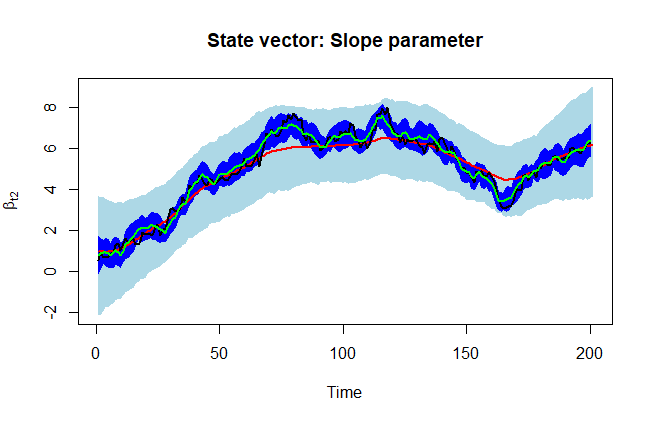
\includegraphics[width=340pt, height=200pt]{Chapters/chapter8/figures/SimSSreg.png}
	\caption[List of figure caption goes here]{Simulation: Dynamic linear model.}\label{fig1}
\end{figure} 

\textbf{Example: Effects of inflation on interest rate I}

We use the dataset \textit{16INTDEF.csv} provided by \cite[Chaps.~10]{wooldridge2016introductory} to study the effects of inflation on the interest rate. The specification is 
\[
\Delta i_t = \beta_{t1} + \beta_{t2}\Delta \text{inf}_t + \beta_{t3}\Delta \text{def}_t + \mu_t
\]
and 
\[
\bm{\beta}_t = \bm{\beta}_{t-1} + \bm{w}_t,
\]
where $\Delta z_t = z_t - z_{t-1}$ is the difference operator, $i_t$ is the three-month T-bill rate, $\text{inf}_t$ is the annual inflation rate based on the consumer price index (CPI), and $\text{def}_t$ is the federal budget deficit as a percentage of gross domestic product (GDP) from 1948 to 2003 in the USA. In addition, $\mu_t \sim N(0, \sigma^2)$ and $\bm{w}_t \sim N(\bm{0}, \text{diag}\{\omega_1^2, \omega_2^2\})$. We assume inverse-gamma distributions for the priors of the scale parameters and set 12,000 MCMC iterations, 2,000 as burn-in, and 10 as the thinning parameter.

The following code shows how to perform this application. We use the variance of the recursive estimation of OLS to set the hyperparameters of the inverse-gamma distribution for the variances of $\bm{w}_t$, and the OLS estimate of the variance of the model to set the hyperparameters of the distribution of $\sigma^2$. Note that, as we are using the function \textit{dlmGibbsDIG} from the \textit{dlm} package, the hyperparameters are set in terms of precision parameters.

Figure \ref{fig2} shows the posterior results of the effect of inflation on the interest rate. This is a fan chart indicating deciles from 10\% to 90\%. The red shaded area shows the range around the median value, and the black line represents the mean value of the state associated with the annual change in inflation. We see that the annual changes in interest rates are weakly positively related to annual changes in inflation.

\begin{tcolorbox}[enhanced,width=4.67in,center upper,
	fontupper=\large\bfseries,drop shadow southwest,sharp corners]
	\textit{R code. Dynamic linear model: Effects of inflation on interest rate}
	\begin{VF}
		\begin{lstlisting}[language=R]
rm(list = ls()); set.seed(010101)
DataIntRate <- read.csv("https://raw.githubusercontent.com/besmarter/BSTApp/refs/heads/master/DataApp/16INTDEF.csv", sep = ",", header = TRUE, quote = "")
attach(DataIntRate); Xt <- cbind(diff(inf), diff(def))
K <- dim(Xt)[2] + 1; yt <- diff(i3)
T <- length(yt); RegLS <- lm(yt ~ Xt)
SumRegLS <- summary(RegLS); SumRegLS; SumRegLS$sigma^2  
# Recursive OLS
Bp <- matrix(RegLS$coefficients, T, K, byrow = TRUE)
S <- 20
for(t in S:T){
	RegLSt <- lm(yt[1:t] ~ Xt[1:t,])
	Bp[t,] <- RegLSt$coefficients 
}
VarBp <- var(Bp)
# State space model
ModelReg <- function(par){
	Mod <- dlm::dlmModReg(Xt, dV = exp(par[1]), dW = exp(par[2:(K+1)]), m0 = RegLS$coefficients,
	C0 = diag(VarBp))
	return(Mod)
}
MCMC <- 12000; burnin <- 2000; thin <- 10
a.y <- (SumRegLS$sigma^2)^(-1); b.y <- 10*a.y; a.theta <- (max(diag(VarBp)))^(-1); b.theta <- 10*a.theta 
gibbsOut <- dlm::dlmGibbsDIG(yt, mod = dlm::dlmModReg(Xt), a.y = a.y, b.y = b.y, a.theta = a.theta, b.theta = b.theta, n.sample = MCMC, thin = 5, save.states = TRUE)
B2t <- matrix(0, MCMC - burnin, T + 1)
for(t in 1:(T+1)){
	B2t[,t] <- gibbsOut[["theta"]][t,2,-c(1:burnin)] 
}
dV <- coda::mcmc(gibbsOut[["dV"]][-c(1:burnin)])
dW <- coda::mcmc(gibbsOut[["dW"]][-c(1:burnin),])
summary(dV); summary(dW)
plot(dV); plot(dW)
library(fanplot); library(latex2exp)
df <- as.data.frame(B2t)
plot(NULL, main="Percentiles", xlim = c(1, T+1), ylim = c(-1, 2), xlab = "Time", ylab = TeX("$\\beta_{t1}$"))
fan(data = df); lines(colMeans(B2t), col = "black", lw = 2)
abline(h=0, col = "blue")
\end{lstlisting}
	\end{VF}
\end{tcolorbox}

\begin{figure}[!h]
	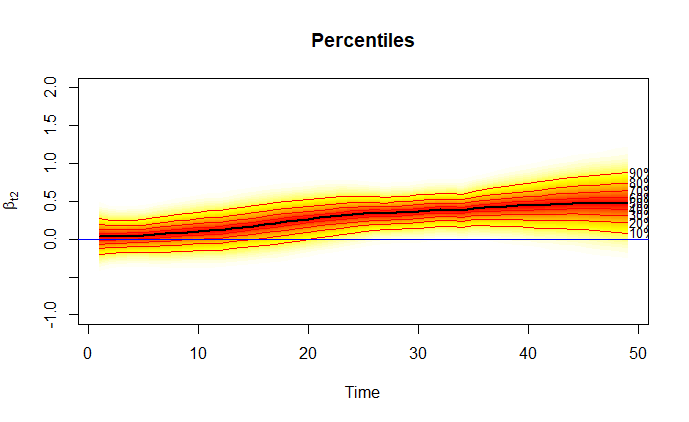
\includegraphics[width=340pt, height=200pt]{Chapters/chapter8/figures/IntInf.png}
	\caption[List of figure caption goes here]{Effects of inflation on interest rate: Dynamic linear model.}\label{fig2}
\end{figure}


We can extend the \textit{dynamic linear model} with \textit{random walk states} to take into account time invariant location parameters. In particular, we follow \cite{de1995simulation}, who propose the \textit{simulation smoother}. This algorithm overcomes some shortcomings of the FFBS algorithm, such as slow convergence and computational overhead. We focus on the case $M=1$, 
\begin{align}
	{y}_t&=\bm{z}_t^{\top}\bm{\alpha}+\bm{x}_t^{\top}\bm{\beta}_t+\bm{h}_t^{\top}\bm{\epsilon}_t,& t=1,2,\dots,T. & \text{   (Observation equation)}\label{DeJongObs}\\
	\bm{\beta}_t&=\bm{\beta}_{t-1}+\bm{H}_t\bm{\epsilon}_t, & t=1,2,\dots,T. & \text{   (States equations)}\label{DeJongSt},
\end{align}
where $\bm{z}_t$ and $\bm{x}_t$ are $L$-dimensional and $K$-dimensional vectors of regressors associated with time-invariant and time-varying parameters, respectively, $\bm{h}_t$ is a vector of dimension $1+K$, $\bm{H}_t$ is a matrix of dimension $K\times (1+K)$, $\bm{\beta}_0=\bm{0}$ and $\bm{\epsilon}_t\sim N(\bm{0}_{1+K},\sigma^2\bm{I}_{1+K})$.

Observe that this specification encompasses Equations \ref{eq1Obs} and \ref{eq1St} setting $\bm{\epsilon}_t=[\mu_t \ \bm{w}_t^{\top}]^{\top}$, $\bm{h}_t=[1 \ 0 \ \dots \ 0]$, $\bm{H}_t=[\bm{0}_K \ \bm{U}_{K\times K}]$ such that $\text{diag}\left\{\omega_1^2 \ \dots \ \omega_K^2\right\}=\sigma^2\bm{U}\bm{U}^{\top}$, $\bm{\alpha}=\bm{0}$, and $\bm{h}_t\bm{H}_t^{\top}=\bm{0}_{K}$.

The nice idea of \cite{de1995simulation} was to propose an efficient algorithm to get draws from $\bm{\eta}_t=\bm{F}_t\bm{\epsilon}_t$, where the most common choice is $\bm{F}_t=\bm{H}_t$, which means drawing samples from the perturbations of the states, and then, recovering the states from Equation \ref{DeJongSt} and $\bm{\beta}_0=\bm{0}$. \cite{de1995simulation} present a more general version of the \textit{state space model} that the one presented here. 

Using the system given by Equations \ref{DeJongObs} and \ref{DeJongSt}, $\bm{F}_t=\bm{H}_t$ and $\bm{h}_t\bm{H}_t^{\top}=\bm{0}_{K}$, the \textit{filtering} recursions are given by $e_t=Y_t-\bm{z}_t^{\top}\bm{\alpha}-\bm{x}_t^{\top}\bm{b}_{t-1}$, ${q}_t=\bm{x}_t^{\top}\bm{B}_{t-1}\bm{x}_t+\bm{h}_t^{\top}\bm{h}_t$, $\bm{K}_t=\bm{B}_{t-1}\bm{x}_tq_t^{-1}$, $\bm{b}_t=\bm{b}_{t-1}+\bm{K}_t e_t$, and $\bm{B}_t=\bm{B}_{t-1}-\bm{B}_{t-1}\bm{x}_t\bm{K}_t^{\top}+\bm{H}_t\bm{H}_t^{\top}$, where $\bm{b}_0=\bm{0}$ and $\bm{B}_0=\bm{H}_0\bm{H}_0^{\top}$. See system 2 in \cite{de1995simulation} for a more general case. We should save $e_t$ (innovation vector), $q_t$ (scale innovation variance) and $\bm{K}_t$ (\textit{Kalman gain}) from this recursion. 

Then, setting $\bm{r}_T=0$ and $\bm{M}_T=\bm{0}$, we run backwards from $t=T-1, T-2, \dots, 1$, the following recursions: $\bm{\Lambda}_{t+1}=\bm{H}_{t+1}\bm{H}_{t+1}^{\top}$, $\bm{C}_{t+1}=\bm{\Lambda}_{t+1}-\bm{\Lambda}_{t+1}\bm{M}_{t+1}\bm{\Lambda}_{t+1}^{\top}$, $\bm{\xi}_{t+1}\sim N(\bm{0}_K,\sigma^2\bm{C}_{t+1})$, $\bm{L}_{t+1}=\bm{I}_K-\bm{K}_{t+1}\bm{x}_{t+1}^{\top}$, $\bm{V}_{t+1}=\bm{\Lambda}_{t+1}\bm{M}_{t+1}\bm{L}_{t+1}$, $\bm{r}_{t}=\bm{x}_{t+1} e_{t+1}/q_{t+1} + \bm{L}_{t+1}^{\top}\bm{r}_{t+1}-\bm{V}_{t+1}^{\top}\bm{C}_{t+1}^{-1}\bm{\xi}_{t+1}$, $\bm{M}_{t}=\bm{x}_{t+1}\bm{x}_{t+1}^{\top}/q_{t+1}+\bm{L}_{t+1}^{\top}\bm{M}_{t+1}\bm{L}_{t+1}+\bm{V}_{t+1}^{\top}\bm{C}_{t+1}^{-1}\bm{V}_{t+1}$, and $\bm{\eta}_{t+1}=\bm{\Lambda}_{t+1}\bm{r}_{t+1}+\bm{\xi}_{t+1}$. \cite{de1995simulation} show that $\bm{\eta}=[\bm{\eta}_1^{\top} \ \dots \ \bm{\eta}_T^{\top}]^{\top}$ is drawn from $p(\bm{H}_t\bm{\epsilon}_t\mid y_t,\bm{x}_t,\bm{z}_t,\bm{h}_t,\bm{H}_t,\bm{\alpha},\sigma^2, t=1,2,\dots,T)$. Thus, we can recover $\bm{\beta}_t$ using \ref{DeJongSt} and $\bm{\beta}_0=\bm{0}_K$.

We assume in the model given by Equations \ref{DeJongObs} and \ref{DeJongSt} that $\bm{h}_t=[1 \ 0 \ \dots \ 0]^{
\top}$ and $\bm{H}_t=[\bm{0}_K \ \text{diag}\left\{1/\tau_1\dots1/\tau_K\right\}]$, and then perform Bayesian inference assuming independent priors, that is, $\pi(\bm{\beta}_0,\bm{\alpha},\sigma^2,\bm{\tau})=\pi(\bm{\beta}_0)\pi(\bm{\alpha})\pi(\sigma^2)\prod_{k=1}^K\pi(\tau_k^2)$ where $\sigma^2\sim IG(\alpha_0/2,\delta_0/2)$, $\tau_k^2\sim G(v_{0}/2,v_{0}/2)$, $k=1,\dots,K$, $\bm{\alpha}\sim N(\bm{a}_0,\bm{A}_0)$ and $\bm{\beta}_0\sim N(\bm{b}_0,\bm{B}_0)$. The conditional posterior distributions are $\sigma^2\mid \bm{y},\bm{X},\bm{Z},\bm{\beta}_{0:T},\bm{\alpha},\bm{\tau}\sim IG(\alpha_{n}/2,\delta_n/2)$, where $\delta_n=\sum_{t=1}^T\left[(\bm{\beta}_t-\bm{\beta}_{t-1})^{\top}\bm{\Psi}(\bm{\beta}_t-\bm{\beta}_{t-1})+(y_t-\bm{z}_t^{\top}\bm{\alpha}-\bm{x}_t^{\top}\bm{\beta}_t)^{\top}(y_t-\bm{z}_t^{\top}\bm{\alpha}-\bm{x}_t^{\top}\bm{\beta}_t)\right]+\delta_0$ and  $\alpha_{n}=T(K+1)+\alpha_0$, $\bm{\tau}=[\tau_1 \ \dots \ \tau_K]$, $\bm{\Psi}=\text{diag}\left\{\tau_1^2,\dots,\tau_K^2\right\}$, and $\tau_k^2\mid \bm{y},\bm{X},\bm{Z},\bm{\beta}_{0:T},\sigma^2\sim G(v_{1n}/2,v_{2kn}/2)$, where $v_{1n}=T+v_{0}$ and $v_{2kn}=\sigma^{-2}\sum_{t=1}^T(\bm{\beta}_{t,k}-\bm{\beta}_{t-1,k})^2+v_{0}$, and $\bm{\alpha}\mid \bm{y},\bm{X},\bm{Z},\sigma^2,\bm{\beta}_{1:T},\bm{\tau}\sim N(\bm{a}_n,\bm{A}_n)$, where $\bm{A}_n=(\bm{A}_0^{-1}+\sigma^{-2}\sum_{t=1}^T\bm{z}_t\bm{z}_t^{\top})^{-1}$ and $\bm{a}_n=\bm{A}_n(\bm{A}_0^{-1}\bm{a}_0+\sigma^{-2}\sum_{t=1}^T\bm{z}_t(y_t-\bm{x}_t^{\top}\bm{\beta}_t))$. The vector of the dependent variable is $\bm{y}$, and all regressors are in $\bm{X}$ and $\bm{Z}$.

We can see that all the previous posterior distributions are conditional on the state vector $\bm{\beta}_{0:T}$, which can be sampled using the \textit{simulation smoother} algorithm, conditional on draws of the time-invariant parameters. Thus, the \textit{state space model} provides an excellent illustration of the modular nature of the Bayesian framework, where performing inference on more complex models often simply involves adding new blocks to an MCMC algorithm. This means we can break down a complex inferential problem into smaller, more manageable parts, which is a ``divide and conquer" approach. This is possible due to the structure of the conditional posterior distributions. Exercise 3 asks you to perform a simulation of the model given by Equations \ref{DeJongObs} and \ref{DeJongSt}, and to program the MCMC algorithm, including the \textit{simulation smoother}.

\section{ARMA processes}\label{sec82}

Since the seminal work of \cite{box_jenkins_1976}, autoregressive moving average (ARMA) models have become ubiquitous in time series analysis. Thus, we present a brief introduction to these models in this section.

Let's start with the linear Gaussian model with autorregresive errors,
\begin{align}
	y_t & = \bm{x}_t^{\top}\bm{\beta}+\mu_t\label{eq1}\\
	\phi(L)\mu_t & = \epsilon_t \label{eq2}, 
\end{align}
where $\bm{x}_t$ is a $K$-dimensional vector of regressors, $\epsilon_t \stackrel{iid}{\sim} N(0,\sigma^2)$, $\phi(L)=1-\phi_1L-\phi_2L^2-\dots-\phi_pL^p$ is a polynomial in the lag operator ($L$), where $Lz_t=z_{t-1}$, and in general, $L^rz_t=z_{t-r}$.

Thus, we see that stochastic error $\mu_t$ follows an \textit{autoregressive process of order $p$}, that is, $\mu_t\sim AR(p)$. It is standard practice to assume that $\mu_t$ is second-order stationary, this implies that the mean, variance and autocovariance of $\mu_t$ are finite and independent of $t$ and $s$, although $\mathbb{E}[\mu_t\mu_s]$ may depend on $|t-s|$. Then, all roots of $\phi(L)$ lie outside the unit circle, for instance, given an $AR(1)$, then, $1-\phi_1L=0$, implies, $L=1/\phi_1$ such that  $|\phi_1|<0$ for the process being second-order stationary.

The likelihood function conditional on the first $p$ observations is
\begin{align*}
	p(y_{p+1},\dots,y_T\mid y_{p},\dots,y_1,\bm{\theta})&=\prod_{t=p+1}^{T}p(y_t\mid \mathcal{I}_{t-1},\bm{\theta})\\
	&\propto \sigma^{-(T-p)}\exp\left\{-\frac{1}{2\sigma^2}\sum_{t=p+1}^T(y_t-\hat{y}_{t\mid t-1,\bm{\theta}})^2\right\},
\end{align*} 
where $\mathcal{I}_{t-1}$ is the past information, $\bm{\theta}$ collects all parameters ($\bm{\beta}, \phi_1,\dots,\phi_p, \sigma^2$), and $\hat{y}_{t\mid t-1,\bm{\theta}}=(1-\phi(L))y_t+\phi(L)\bm{x}^{\top}\bm{\beta}$.

We can see that multiplying the first expression in Equation \ref{eq1} by $\phi(L)$, we can express the model as 
\begin{align}\label{eq3}
	y_t^*=\bm{x}_t^{*\top}\bm{\beta}+\epsilon_t
\end{align}
where $y_t^*=\phi(L)Y_t$ and $\bm{x}_t^{*}=\phi(L)\bm{x}_t$.

Thus, collecting all observations $t=p+1,p+2,\dots,T$, we have $\bm{y}^*=\bm{X}^*\bm{\beta}+\bm{\epsilon}$, where $\bm{\epsilon}\sim N(\bm{0},\sigma^2\bm{I}_{T-p})$, $\bm{y}^*$ is a $T-p$ dimensional vector, and $\bm{X}^*$ is a $(T-p)\times K$ dimensional matrix.

Assuming that $\bm{\beta}\mid \sigma\sim N(\bm{\beta}_0,\sigma^2\bm{B}_0)$, $\sigma^2\sim IG(\alpha_0/2,\delta_0/2)$ and $\bm{\phi}\sim N(\bm{\phi}_0,\bm{\Phi}_0)\mathbbm{1}(\bm{\phi}\in S_{\bm{\phi}})$, where $S_{\bm{\phi}}$ is the stationary region of $\bm{\phi}=[\phi_1 \ \dots \ \phi_p]^{\top}$. Then, Equation \ref{eq3} implies that $\bm{\beta}\mid \sigma^2,\bm{\phi},\bm{y},\bm{X}\sim N(\bm{\beta}_n, \sigma^2{\bm{B}}_n)$, where $\bm{B}_n = (\bm{B}_0^{-1} + \bm{X}^{*\top}\bm{X}^{*})^{-1}$ and $\bm{\beta}_n = \bm{B}_n(\bm{B}_0^{-1}\bm{\beta}_0 + \bm{X}^{*\top}\bm{y}^{*})$. In addition, $\sigma^2\mid \bm{\beta},\bm{\phi},\bm{y},\bm{X}\sim IG(\alpha_n/2,\delta_n/2)$ where $\alpha_n=\alpha_0+T-p$ and $\delta_n=\delta_0+(\bm{y}^*-\bm{X}^{*}\bm{\beta})^{\top}(\bm{y}^*-\bm{X}^{*}\bm{\beta})+(\bm{\beta}-\bm{\beta}_0)\bm{B}_0^{-1}(\bm{\beta}-\bm{\beta}_0)$. Thus, the previous conditional posterior distributions imply that we can use a Gibbs sampling algorithm to perform inference of these parameters \cite{chib1993bayes}.

We know from Equation \ref{eq1} that $\mu_t=y_t-\bm{x}_t^{\top}\bm{\beta}$, from Equation \ref{eq2} that $\mu_t=\phi_1\mu_{t-1}+\dots+\phi_p\mu_{t-p}+\epsilon_t$, $t=p+1,\dots,T$. In matrix notation $\bm{\mu}=\bm{U}\bm{\phi}+\bm{\epsilon}$, where $\bm{\mu}$ is a $T-p$ dimensional vector, $\bm{U}$ is a $(T-p)\times p$ matrix whose $t$-th row is $[\mu_{t-1} \ \dots \ \mu_{t-p}]$. Thus, the posterior distribution of $\bm{\phi}\mid \bm{\beta},\sigma^2,\bm{y},\bm{X}$ is $N(\bm{\phi}_n, \bm{\Phi}_n)\mathbbm{1}(\bm{\phi}\in S_{\bm{\phi}})$, where $\bm{\Phi}_n=(\bm{\Phi}_0^{-1}+\sigma^{-2}\bm{U}^{\top}\bm{U})$ and $\bm{\phi}_n=\bm{\Phi}_n(\bm{\Phi}_0^{-1}\bm{\phi}_0+\sigma^{-2}\bm{U}^{\top}\bm{\mu})$ (see Exercise 4).

Drawing from the model under the stationarity restriction is straightforward: we simply sample from the multivariate normal distribution and discard draws that do not satisfy the stationarity condition. The proportion of draws that meet this restriction represents the conditional probability that the process is stationary.\\

\textbf{Example: Effects of inflation on interest rate II}

We specify a \textit{dynamic linear model} in the example of the effects of inflation on interest rates to account for a potential dynamic relationship. However, we can introduce dynamics in this model by assuming 
\[
\Delta i_t = \beta_{1} + \beta_{2} \Delta inf_t + \beta_{3} \Delta def_t + \mu_t,
\]
where \(\mu_t = \phi \mu_{t-1} + \epsilon_t\). This leads to the model:
\[
\Delta i_t = \beta_{1}(1-\phi_1) + \phi_1 \Delta i_{t-1} + \beta_{2}(\Delta inf_t - \phi_1 \Delta inf_{t-1}) + \beta_{3}(\Delta def_t - \phi_1 \Delta def_{t-1}) + \epsilon_t.
\]
Thus, we again use the dataset \textit{16INTDEF.csv} provided by \cite[Chaps.~10]{wooldridge2016introductory} to illustrate linear regressions with $AR(1)$ errors.

The following code demonstrates how to implement this application using vague priors, assuming \(\alpha_0 = \delta_0 = 0.01\), \(\bm{\beta}_0 = \bm{0}\), \(\bm{B}_0 = \bm{I}\), \(\bm{\phi}_0 = \bm{0}\), and \(\bm{\Phi}_0 = \bm{I}\). We use 15,000 MCMC iterations, with a burn-in of 5,000 and a thinning parameter of 5.

\begin{tcolorbox}[enhanced,width=4.67in,center upper,
	fontupper=\large\bfseries,drop shadow southwest,sharp corners]
	\textit{R code. AR(1) model: Effects of inflation on interest rate}
	\begin{VF}
		\begin{lstlisting}[language=R]
rm(list = ls())
set.seed(010101)
DataIntRate <- read.csv("https://raw.githubusercontent.com/besmarter/BSTApp/refs/heads/master/DataApp/16INTDEF.csv", sep = ",", header = TRUE, quote = "")
attach(DataIntRate)
yt <- diff(i3); ytlag <- dplyr::lag(yt, n = 1)
T <- length(yt)
Xt <- cbind(diff(inf), diff(def)); Xtlag <- dplyr::lag(Xt, n = 1)
K <- dim(Xt)[2] + 1
Reg <- lm(yt ~ ytlag + I(Xt[,-1] - Xtlag))
SumReg <- summary(Reg); SumReg
PostSig2 <- function(Beta, Phi){
	Xstar<- matrix(NA, T-1, K - 1)
	ystar <- matrix(NA, T-1, 1)
	for(t in 2:T){
		Xstar[t-1,] <- Xt[t,] - Phi*Xt[t-1,]
		ystar[t-1,] <- yt[t] - Phi*yt[t-1]
	}
	Xstar <- cbind(1, Xstar)
	an <- T - 1 + a0
	dn <- d0 + t(ystar - Xstar%*%Beta)%*%(ystar - Xstar%*%Beta) + t(Beta - b0)%*%B0i%*%(Beta - b0)
	sig2 <- invgamma::rinvgamma(1, shape = an/2, rate = dn/2)
	return(sig2)
}
PostBeta <- function(sig2, Phi){
	Xstar<- matrix(NA, T-1, K - 1)
	ystar <- matrix(NA, T-1, 1)
	for(t in 2:T){
		Xstar[t-1,] <- Xt[t,] - Phi*Xt[t-1,]
		ystar[t-1,] <- yt[t] - Phi*yt[t-1]
	}
	Xstar <- cbind(1, Xstar)
	XtXstar <- t(Xstar)%*%Xstar
	Xtystar <- t(Xstar)%*%ystar
	Bn <- solve(B0i + XtXstar)
	bn <- Bn%*%(B0i%*%b0 + Xtystar)
	Beta <- MASS::mvrnorm(1, bn, sig2*Bn)
	return(Beta)
}
PostPhi <- function(sig2, Beta){
	u <- yt - cbind(1,Xt)%*%Beta
	U <- u[-T]
	ustar <- u[-1]
	UtU <- t(U)%*%U
	Utu <- t(U)%*%ustar
	Phin <- solve(Phi0i + sig2^(-1)*UtU)
	phin <- Phin%*%(Phi0i%*%phi0 + sig2^(-1)*Utu)
	Phi <- truncnorm::rtruncnorm(1, a = -1, b = 1, mean = phin, sd = Phin^0.5)
	return(Phi)
}
		\end{lstlisting}
	\end{VF}
\end{tcolorbox}


\begin{tcolorbox}[enhanced,width=4.67in,center upper,
	fontupper=\large\bfseries,drop shadow southwest,sharp corners]
	\textit{R code. AR(1) model: Effects of inflation on interest rate}
	\begin{VF}
		\begin{lstlisting}[language=R]
# Hyperparameters
d0 <- 0.01; a0 <- 0.01
b0 <- rep(0, K); c0 <- 1; 
B0 <- c0*diag(K); B0i <- solve(B0)
phi0 <- 0; Phi0 <- 1; Phi0i <- 1/Phi0
# MCMC parameters
mcmc <- 15000
burnin <- 5000
tot <- mcmc + burnin
thin <- 1
PostBetas <- matrix(0, mcmc+burnin, K)
PostSigma2s <- rep(0, mcmc+burnin)
PostPhis <- rep(0, mcmc+burnin)
Beta <- rep(0, K); Phi <- 0
sig2 <- SumReg$sigma^2; Phi <- SumReg$coefficients[2,1]
Beta <- SumReg$coefficients[c(1,3,4),1]
pb <- txtProgressBar(min = 0, max = tot, style = 3)
for(s in 1:tot){
	sig2 <- PostSig2(Beta = Beta, Phi = Phi)
	PostSigma2s[s] <- sig2
	Beta <- PostBeta(sig2 = sig2, Phi = Phi)
	PostBetas[s,] <- Beta
	Phi <- PostPhi(sig2 = sig2, Beta = Beta)
	PostPhis[s] <- Phi
	setTxtProgressBar(pb, s)
}
close(pb)
keep <- seq((burnin+1), tot, thin)
PosteriorBetas <- coda::mcmc(PostBetas[keep,])
summary(PosteriorBetas)
PosteriorSigma2 <- coda::mcmc(PostSigma2s[keep])
summary(PosteriorSigma2)
PosteriorPhi <- coda::mcmc(PostPhis[keep])
summary(PosteriorPhi)
dfBinf <- as.data.frame(PosteriorBetas[,2])
# Basic density
library(ggplot2)
p <- ggplot(dfBinf, aes(x=var1)) + 
geom_density(color="darkblue", fill="lightblue") +
geom_vline(aes(xintercept=mean(var1)), color="blue", linetype="dashed", linewidth=1) +
geom_vline(aes(xintercept=quantile(var1, 0.025)), color="red", linetype="dashed", linewidth=1) +
geom_vline(aes(xintercept=quantile(var1, 0.975)), color="red", linetype="dashed", linewidth=1) +
labs(title="Density effect of inflation on interest rate", x="Effect of inflation", y = "Density")
\end{lstlisting}
	\end{VF}
\end{tcolorbox}

Figure \ref{fig3} shows the posterior density plot of the effects of inflation rate on interest rate. The posterior mean of this coefficient is approximately 0.25, and the credible interval at 95\% is (0, 0.46), which indicates again that the annual changes in interest rate are weakly positive related to annual changes in inflation (see Figure \ref{fig2} as reference). 

\begin{figure}[!h]
	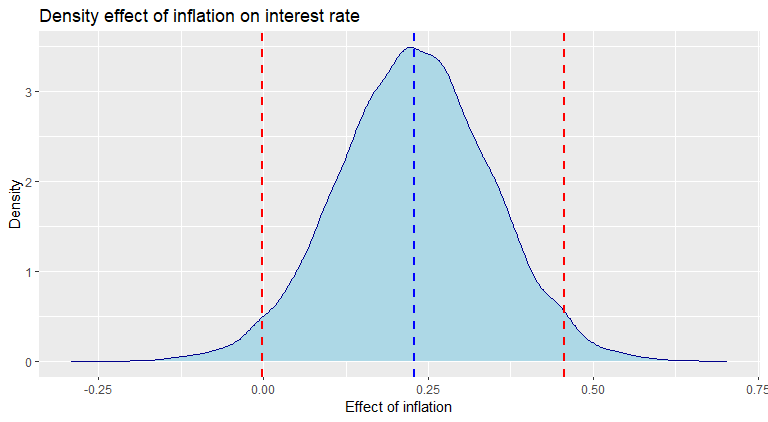
\includegraphics[width=340pt, height=200pt]{Chapters/chapter8/figures/InfInt.png}
	\caption[List of figure caption goes here]{Density: Effects of inflation on interest rate.}\label{fig3}
\end{figure} 

Observe that the previous setting encompasses the particular relevant case  $y_t\sim AR(p)$, it is just omitting the covariates such that $y_t=\mu_t$. \cite{chib1994bayes} extend the Bayesian inference of linear regression with $AR(p)$ errors to $ARMA(p,q)$ errors using a \textit{state-space} representation. 

Setting $y_t=\mu_t$ such that $y_t=\sum_{s=1}^{p}\phi_jy_{t-s}+\sum_{s=1}^{q}\theta_s \epsilon_{t-s}+\epsilon_t$, letting $r=\max \left\{p,q+1\right\}$, $\phi_s=0$ for $s>p$ and $\theta_s=0$ for $s>q$, and defining $\bm{x}^{\top}=[1 \ 0 \ \dots \ 0]$, and $\bm{H}=[1 \ \psi_1 \ \dots \ \psi_{r-1}]^{\top}$ $r$-dimensional vectors, and 
\begin{align*}
	\bm{G}=\begin{bmatrix}
		\phi_1 & 1 & 0 & \dots & 0\\
		\phi_2 & 0 & 1 & \dots & 0\\
		\vdots & \vdots & \ddots &  &\\
		\phi_{r-1} & 0 & 0 & \dots & 1\\
		\phi_r & 0 & 0 & \dots & 0\\
	\end{bmatrix} = \begin{bmatrix}
		\phi_1 & \vdots &  &  & \\
		\phi_2 & \vdots &  & \bm{I}_{r-1}  & \\
		\vdots & \vdots &  &  &\\
		\dots & \dots & \dots & \dots & \dots\\
		\phi_r & 0 & 0 & \dots & 0\\
	\end{bmatrix},
\end{align*} 
which is a $r\times r$ dimensional matrix, and give the \textit{state} vector $\bm{\beta}_t=[\beta_{1,t} \ \beta_{2,t} \ \dots \ \beta_{r,t}]^{\top}$, the $ARMA$ model has the following representation:
\begin{align*}
	y_t&=\bm{x}^{\top}\bm{\beta}_t\\
	\bm{\beta}_t &= \bm{G}\bm{\beta}_{t-1}+\bm{H}\epsilon_{t}.
\end{align*}

This is a \textit{dynamic linear model} where $\bm{\Sigma}_t=0$, and $\bm{\Omega}_t=\sigma^2\bm{H}\bm{H}^{\top}$ (see \cite{petris2009dynamic,chib1994bayes}).

A notable advantage of the \textit{state-space} representation of the $ARMA$ model is that the evaluation of the likelihood can be performed efficiently using the recursive laws. Extensions to autoregressive integrated moving average $ARIMA(p,d,q)$ models are discussed in \cite[Chap.~3]{petris2009dynamic}. In $ARIMA(p,d,q)$ models, $d$ refers to the level of integration (or differencing) required to eliminate the stochastic trend in a time series (see \cite[Chap.~4]{enders_2014} for details).\\

\textbf{Example: $AR(2)$ process}

Let's see the \textit{state-space} representation of a stationary $AR(2)$ process with intercept, that is, $y_t=\mu+\phi_1y_{t-1}+\phi_2y_{t-2}+\epsilon_t$, where $\epsilon_t\sim N(0,\sigma^2)$. Thus, $\mathbb{E}[y_t]=\frac{\mu}{1-\phi_1-\phi_2}$, and variance $Var[y_t]=\frac{\sigma^2(1-\phi_2)}{1-\phi_2-\phi_1^2-\phi_1^2\phi_2-\phi_2^2+\phi_2^3}$.

In addition, we can proof that setting $z_t=Y_t-\bar{\mu}$, we have $z_t=\phi_1z_{t-1}+\phi_2z_{t-2}+\epsilon_t$ where $\mathbb{E}[z_t]=0$, and these are equivalent representations (see Exercise 5). Then, setting  $\bm{x}^{\top}=[1 \ 0]$, $\bm{H}=[1 \ 0]^{\top}$, $\bm{G}=\begin{bmatrix}
	\phi_1 & 1\\
	\phi_2 & 0 \\
\end{bmatrix}$, $\bm{\beta}_t=[\beta_{t1} \ \beta_{t2}]^{\top}$, $\bm{\Sigma}_t=0$ and $\bm{\Omega}_t=\sigma^2$ we have
\begin{align*}
	z_t&=\bm{x}^{\top}\bm{\beta}_t& \text{(Observation equation)}\\
	\bm{\beta}_t&=\bm{G}\bm{\beta}_{t-1}+\bm{H}{\epsilon}_t & \text{(States equations)}.
\end{align*}

We use the function \textit{stan\_sarima} from the package \textit{bayesforecast} to perform Bayesian inference in $ARMA$ models in our GUI. The following code shows how to simulate an $AR(2)$ process, and perform Bayesian inference using this function.

\begin{tcolorbox}[enhanced,width=4.67in,center upper,
	fontupper=\large\bfseries,drop shadow southwest,sharp corners]
	\textit{R code. Simulation and inference: AR(2) model}
	\begin{VF}
		\begin{lstlisting}[language=R]
rm(list = ls()); set.seed(010101)
T <- 200; mu <- 0.5 
phi1 <- 0.5; phi2 <- 0.3; sig <- 0.5
Ey <- mu/(1-phi1-phi2); Sigy <- sig*((1-phi2)/(1-phi2-phi1^2-phi2*phi1^2-phi2^2+phi2^3))^0.5 
y <- rnorm(T, mean = Ey, sd = Sigy)
e <- rnorm(T, mean = 0, sd = sig)
for(t in 3:T){
	y[t] <- mu + phi1*y[t-1] + phi2*y[t-2] + e[t]
}
mean(y); sd(y)
y <- ts(y, start=c(1820, 1), frequency=1)
plot(y)
iter <- 10000; burnin <- 5000; thin <- 1; tot <- iter + burnin
library(bayesforecast)
sf1 <- bayesforecast::stan_sarima(y, order = c(2, 0, 0), prior_mu0 = normal(0, 1),
prior_ar = normal(0, 1), prior_sigma0 = inverse.gamma(0.01/2, 0.01/2),
seasonal = c(0, 0, 0), iter = tot, warmup = burnin, chains = 1)
keep <- seq(burnin+1, tot, thin)
Postmu <- sf1[["stanfit"]]@sim[["samples"]][[1]][["mu0"]][keep]
Postsig <- sf1[["stanfit"]]@sim[["samples"]][[1]][["sigma0"]][keep]
Postphi1 <- sf1[["stanfit"]]@sim[["samples"]][[1]][["ar0[1]"]][keep]
Postphi2 <- sf1[["stanfit"]]@sim[["samples"]][[1]][["ar0[2]"]][keep]
Postdraws <- coda::mcmc(cbind(Postmu, Postsig, Postphi1, Postphi2))
summary(Postdraws)
Quantiles for each variable:
            	2.5%    25%    50%    75%  97.5%
Postmu   0.39914 0.5732 0.6625 0.7518 0.9346
Postsig  0.47696 0.5071 0.5248 0.5439 0.5829
Postphi1 0.42384 0.5159 0.5634 0.6089 0.6979
Postphi2 0.06034 0.1456 0.1920 0.2361 0.3286
plot(Postdraws)
\end{lstlisting}
	\end{VF}
\end{tcolorbox}
We perform 10000 MCMC iterations plus a burn-in equal 5000 assuming $\sigma^2\sim IG(0.01/2, 0.01/2)$, $\mu\sim N(0, 1)$ and $\phi_k\sim N(0, 1)$, $k=1,2$. The trace plots look well, and all 95\% credible intervals encompass the population values.

Algorithm \ref{alg:ARMA} shows how to perform inference in $ARMA(p,q)$ models using our GUI. See also Chapter \ref{chapGUI} for details regarding the dataset structure. 

\begin{algorithm}[h!]
	\caption{Autoregressive Moving Average ($ARMA$) models}\label{alg:ARMA}
	\begin{algorithmic}[1]  		 			
		\State Select \textit{Time series Model} on the top panel
		\State Select \textit{ARMA} using the left radio button
		\State Upload the dataset selecting first if there is header in the file, and the kind of separator in the \textit{csv} file of the dataset (comma, semicolon, or tab). Then, use the \textit{Browse} button under the \textbf{Choose File} legend
		\State Select MCMC iterations, burn-in and thinning parameters using the \textit{Range sliders}
		\State Set the order of the ARMA model, $p$ and $q$ parameters
		\State Set the frequency: annual (1), quarterly (4), monthly (12), etc
		\State Set the location and scale hyperparameters of the \textit{intercept}, autoregressive ($AR$), moving average ($MA$) and standard deviation. Take into account that there is just one set of hyperparameters for $AR$ and $MA$ coefficients. This step is not necessary as by default our GUI uses non-informative priors
		\State Click the \textit{Go!} button
		\State Analyze results
		\State Download posterior chains and figures (density, autocorrelation and trace plots) using the \textit{Download Results} button
	\end{algorithmic} 
\end{algorithm}

The function \textit{stan\_sarima} uses the \textit{Stan} software \cite{Stan2024}, which in turn employs \textit{Hamiltonian Monte Carlo} (HMC). The following code illustrates how to perform Bayesian inference in the $AR(2)$ model by programming the HMC from scratch. It is important to note that this is only an illustration, as HMC is less efficient than the Gibbs sampler in this example. However, HMC can outperform traditional MCMC algorithms in more complex models, particularly when dealing with high-dimensional probability distributions or when MCMC struggles with poor mixing due to posterior correlation.

In the first block, we perform the simulation by setting $\mu=0.5$, $\phi_1=0.5$, $\phi_2=0.3$, $\sigma=0.25$, and a sample size of 200. We then set the hyperparameters and define the function to calculate the logarithm of the posterior distribution. The model is parametrized using $\tau = \log(\sigma^2)$, such that $\sigma^2=\exp(\tau)$, which avoids issues related to the non-negativity restriction of $\sigma^2$. As a result, we need to account for the Jacobian due to this transformation, specifically $d\sigma^2/d\tau = \exp(\tau)$.

Next, we define the function to compute the gradient vector of the log posterior distribution. It is preferable to calculate the gradient vector analytically, as using finite differences can be computationally expensive. However, it is a good practice to check the analytical calculations by evaluating the function at the maximum posterior estimate, where the function should return values close to 0, or by comparing the results with finite differences at a few evaluation points.

The posterior distribution is given by\footnote{Take into account that we do not consider the first two observations when present the likelihood, this is no an issue when there is a large sample size.}
\begin{align*}
	\pi(\mu,\phi_1,\phi_2,\tau\mid \bm{y})&\propto \prod_{t=3}^T(\exp(\tau))^{-1/2}\exp\left\{-\frac{1}{2\exp(\tau)}(y_t-\mu-\phi_1y_{t-1}-\phi_2y_{t-2})^2\right\}\\
	&\times\exp\left\{-\frac{1}{2\sigma^2_{\mu}}(\mu-\mu_0)^2\right\}\times\exp\left\{-\frac{1}{2\sigma^2_{\phi_1}}(\phi_1-\phi_{10})^2\right\}\\
	&\times\exp\left\{-\frac{1}{2\sigma^2_{\phi_2}}(\phi_2-\phi_{20})^2\right\}\times\exp\left\{-(\alpha_0/2+1)\tau\right\}\exp\left\{-\delta_0/(2\exp(\tau))\right\}\exp(\tau).
\end{align*} 

The components of the gradient vector of the log posterior distribution are given by
\begin{align*}
	\frac{\partial \log(\pi(\mu,\phi_1,\phi_2,\tau\mid \bm{y}))}{\partial\mu}&=\frac{\sum_{t=3}^T(y_t-\mu-\phi_1y_{t-1}-\phi_2y_{t-2})}{\exp(\tau)}-\frac{1}{\sigma_{\mu}^2}(\mu-\mu_0)\\
	\frac{\partial\log(\pi(\mu,\phi_1,\phi_2,\tau\mid \bm{y}))}{\partial\phi_1}&=\frac{\sum_{t=3}^T(y_t-\mu-\phi_1y_{t-1}-\phi_2y_{t-2})y_{t-1}}{\exp(\tau)}-\frac{1}{\sigma_{\phi_1}^2}(\phi_1-\phi_{10})\\
	\frac{\partial\log(\pi(\mu,\phi_1,\phi_2,\tau\mid \bm{y}))}{\partial\phi_2}&=\frac{\sum_{t=3}^T(y_t-\mu-\phi_1y_{t-1}-\phi_2y_{t-2})y_{t-2}}{\exp(\tau)}-\frac{1}{\sigma_{\phi_2}^2}(\phi_2-\phi_{20})\\	\frac{\partial\log(\pi(\mu,\phi_1,\phi_2,\tau\mid \bm{y}))}{\partial\tau}&=-\frac{(T-2)}{2}+\frac{\sum_{t=3}^T(y_t-\mu-\phi_1y_{t-1}-\phi_2y_{t-2})^2}{2\exp(\tau)}\\
	&-(\alpha_0/2+1)+\delta_0/(2\exp(\tau))+1.\\
\end{align*}

Next, we provide the code for the Hamiltonian Monte Carlo, as outlined in Chapter \ref{chap5}. The initial values are set as follows: $\mu=\bar{y}=\frac{1}{T-2}\sum_{t=3}^T y_t$, $\phi_1=\phi_2=0$, and $\tau=\exp\left(\frac{1}{T-2}\sum_{t=3}^T(y_t-\bar{y})^2\right)$, with $M$ being the inverse covariance matrix of the posterior distribution evaluated at its maximum. Additionally, $\epsilon$ is randomly drawn from a uniform distribution between 0 and $2\epsilon_0$, and $L$ is set to the highest integer near $1/\epsilon$, in order to approximately satisfy $L\epsilon=1$, where $\epsilon_0=0.1$.

We can verify that all 95\% credible intervals encompass the population values, and the posterior means are close to the population values. The acceptance rate averages above 65\%, so we should consider increasing the base step ($\epsilon_0$). Furthermore, we do not impose the stationarity conditions on $\phi_1$ and $\phi_2$. Exercise 6 asks to program an HMC that takes these requirements into account.

\begin{tcolorbox}[enhanced,width=4.67in,center upper,
	fontupper=\large\bfseries,drop shadow southwest,sharp corners]
	\textit{R code. Simulation and inference: AR(2) model using Hamiltonian Monte Carlo}
	\begin{VF}
		\begin{lstlisting}[language=R]
# Simulation AR(2)
rm(list = ls()); set.seed(010101); T <- 1000; K <- 4 
mu <- 0.5; phi1 <- 0.5; phi2 <- 0.3; sig <- 0.5 
Ey <- mu/(1-phi1-phi2); Sigy <- sig*((1-phi2)/(1-phi2-phi1^2-phi2*phi1^2-phi2^2+phi2^3))^0.5 
y <- rnorm(T, mean = Ey, sd = Sigy); e <- rnorm(T, mean = 0, sd = sig)
for(t in 3:T){
	y[t] <- mu + phi1*y[t-1] + phi2*y[t-2] + e[t]
}
# Hyperparameters
d0 <- 0.01; a0 <- 0.01; mu0 <- 0; MU0 <- 1
phi0 <- c(0, 0); Phi0 <- diag(2)
# Log posterior multiply by -1 to use optim
LogPost <- function(theta, y){
	mu <- theta[1]; phi1 <- theta[2]; phi2 <- theta[3]
	tau <- theta[4]; sig2 <- exp(tau); logLik <- NULL
	for(t in 3:T){
		logLikt <- dnorm(y[t], mean = mu + phi1*y[t-1] + phi2*y[t-2], sd = sig2^0.5, log = TRUE)
		logLik <- c(logLik, logLikt)
	}
	logLik <- sum(logLik)
	logPrior <- dnorm(mu, mean = mu0, sd = MU0^0.5, log = TRUE) + dnorm(phi1, mean = phi0[1], sd = Phi0[1,1]^0.5, log = TRUE) + dnorm(phi2, mean = phi0[2], sd = Phi0[2,2]^0.5, log = TRUE) + invgamma::dinvgamma(sig2, shape = a0/2, rate = d0/2, log = TRUE)
	logPosterior <- logLik + logPrior + tau
	return(-logPosterior) # Multiply by -1 to minimize using optim
}
theta0 <- c(mean(y), 0, 0, var(y))
Opt <- optim(theta0, LogPost, y = y, hessian = TRUE)
theta0 <- Opt$par; VarPost <- solve(Opt$hessian)
# Gradient log posterior
GradientTheta <- function(theta, y){
	mu <- theta[1]; phi1 <- theta[2]; phi2 <- theta[3]
	tau <- theta[4]; sig2 <- exp(tau); SumLik <- matrix(0, 3, 1)
	SumLik2 <- NULL
	for(t in 3:T){
		xt <- matrix(c(1, y[t-1], y[t-2]), 3, 1)
		SumLikt <- (y[t] - (mu + phi1*y[t-1] + phi2*y[t-2]))*xt
		SumLik2t <- (y[t] - (mu + phi1*y[t-1] + phi2*y[t-2]))^2
		SumLik <- rowSums(cbind(SumLik, SumLikt))
		SumLik2 <- sum(SumLik2, SumLik2t)
	}
	Grad_mu <- SumLik[1]/sig2 - (1/MU0)*(mu - mu0)
	Grad_phi1 <- SumLik[2]/exp(tau) - 1/Phi0[1,1]*(phi1 - phi0[1])
	Grad_phi2 <- SumLik[3]/exp(tau) - 1/Phi0[2,2]*(phi2 - phi0[2])
	Grad_tau <- -(T-2)/2 + SumLik2/(2*exp(tau)) - (a0/2 + 1) + d0/(2*exp(tau)) + 1 
	Grad <- c(Grad_mu, Grad_phi1, Grad_phi2, Grad_tau)
	return(Grad)
}
\end{lstlisting}
	\end{VF}
\end{tcolorbox}

\begin{tcolorbox}[enhanced,width=4.67in,center upper,
	fontupper=\large\bfseries,drop shadow southwest,sharp corners]
	\textit{R code. Simulation and inference: AR(2) model using Hamiltonian Monte Carlo}
	\begin{VF}
		\begin{lstlisting}[language=R]
# Hamiltonian Monte Carlo function
HMC <- function(theta, y, epsilon, M){
	L <- ceiling(1/epsilon)
	Minv <- solve(M); thetat <- theta
	K <- length(thetat)
	mom <- t(mvtnorm::rmvnorm(1, rep(0, K), M))
	logPost_Mom_t <- -LogPost(thetat, y) +  mvtnorm::dmvnorm(t(mom), rep(0, K), M, log = TRUE)  
	for(l in 1:L){
		if(l == 1 | l == L){
			mom <- mom + 0.5*epsilon*GradientTheta(theta, y)
			theta <- theta + epsilon*Minv%*%mom
		}else{
			mom <- mom + epsilon*GradientTheta(theta, y)
			theta <- theta + epsilon*Minv%*%mom
		}
	}
	logPost_Mom_star <- -LogPost(theta, y) +  mvtnorm::dmvnorm(t(mom), rep(0, K), M, log = TRUE)  
	alpha <- min(1, exp(logPost_Mom_star-logPost_Mom_t))
	u <- runif(1)
	if(u <= alpha){
		thetaNew <- c(theta)
	}else{
		thetaNew <- thetat
	}
	rest <- list(theta = thetaNew, Prob = alpha)
	return(rest)
}
# Posterior draws
S <- 1000; burnin <- 1000; thin <- 2; tot <- S + burnin
thetaPost <- matrix(NA, tot, K)
ProbAccept <- rep(NA, tot)
theta0 <- c(mean(y), 0, 0, exp(var(y))) 
M <- solve(VarPost); epsilon0 <- 0.1
pb <- txtProgressBar(min = 0, max = tot, style = 3)
for(s in 1:tot){
	epsilon <- runif(1, 0, 2*epsilon0)
	L <- ceiling(1/epsilon)
	HMCs <- HMC(theta = theta0, y, epsilon, M) 
	theta0 <- HMCs$theta 
	thetaPost[s,] <- HMCs$theta
	ProbAccept[s] <- HMCs$Prob
	setTxtProgressBar(pb, s)
}
close(pb)
keep <- seq((burnin+1), tot, thin)
thetaF <- coda::mcmc(thetaPost[keep,])
summary(thetaF)
summary(exp(thetaF[,K]))
ProbAcceptF <- coda::mcmc(ProbAccept[keep])
summary(ProbAcceptF)
\end{lstlisting}
	\end{VF}
\end{tcolorbox} 
    
\section{Stochastic volatility models}\label{sec83}
A notable example of non-linear and non-Gaussian \textit{state-space models} is stochastic volatility models (SVMs), which are widely used to model the volatility of financial returns. SVMs have gained significant attention due to their flexibility, ability to capture complex dynamics such as asymmetries, and ease of generalization to simultaneously model multiple returns, making them advantageous over generalized autoregressive conditional heteroskedasticity (GARCH) models proposed by \cite{bollerslev_1986}. However, estimating SVMs is more challenging than estimating GARCH models. This is because GARCH models set variance in a deterministic manner, whereas SVMs do so stochastically. Consequently, GARCH models are typically estimated using maximum likelihood methods, while SVMs require Bayesian approaches, adding complexity to the estimation process.

The specification of the stochastic volatility model is given by
\begin{align}
	y_t&=\bm{x}_t^{\top}\bm{\beta}+\exp\left\{0.5h_t\right\}\mu_t& \text{(Observation equation)}\label{eqsvobs}\\
	h_t&=\mu+\phi(h_{t-1}-\mu)+\sigma w_t& \text{(State equation)}\label{eqsvst},
\end{align}
where $y_t$ are the log-returns, $\bm{x}_t$ are controls, $\bm{\beta}$ are time-invariant location parameters, $\mu_t\sim N(0,1)$, $w_t\sim N(0,1)$, $\mu_t\perp w_t$, the initial log-variance process $h_0\sim N(\mu, \sigma^2/(1-\phi^2))$, $\mu$, $\phi$ and $\sigma$ are the level, persistence and standard deviation of the log-variance, respectively.

Given the specification in Equations \ref{eqsvobs} and \ref{eqsvst}, we can write the observation equation as 
\[
\log\left\{(y_t-\bm{x}_t^{\top}\bm{\beta})^2\right\} = h_t + \log(\mu_t^2),
\]
which leads to a linear, but non-Gaussian, \textit{state-space model}. \cite{kastner2014ancillarity} approximate the distribution of $\log(\mu_t^2)$ by a mixture of normal distributions, that is, 
\[
\log(\mu_t^2)\mid l_t \sim N(m_{l_t},s_{l_t}^2),
\]
where $l_t \in \{1, 2, \dots, 10\}$ defines the mixture component indicator at time $t$. Thus, the model can be written as
\[
\log\left\{(y_t-\bm{x}_t^{\top}\bm{\beta})^2\right\} = h_t + \log(\mu_t^2),
\]
and
\[
h_t = \mu + \phi(h_{t-1} - \mu) + \sigma w_t.
\]
This forms a linear and conditionally Gaussian \textit{state-space model}, where
\[
\log\left\{(y_t-\bm{x}_t^{\top}\bm{\beta})^2\right\} = m_{l_t} + h_t + \mu_t^2,
\]
and
\[
\mu_t \sim N(0, s_{l_t}^2).
\]

We use the \textit{stochvol} package in our GUI to perform MCMC inference in the SVMs \cite{hosszejni_kastner_2021}; this package is based on the MCMC algorithms proposed by \cite{kastner2014ancillarity}. The default prior distributions in the \textit{stochvol} package are: 
\[
\bm{\beta} \sim N(\bm{b}_0, \bm{B}_0), \quad \mu \sim N(\mu_0, \sigma_{\mu0}^2), \quad \frac{\phi+1}{2} \sim B(\alpha_0, \beta_0), \quad \sigma^2 \sim G\left(\frac{1}{2}, \frac{1}{2\sigma^2_{\sigma^2}}\right).
\]
The prior distribution for $\phi$ is set to ensure stationarity of the process ($\phi \in (-1,1)$). In most applications, $\phi \approx 1$, so the authors of the package recommend setting $\alpha_0 \gtrsim 5$ and $\beta_0 \approx 1.5$. The prior distribution for $\sigma$ is $ |N(0, \sigma^2_{\sigma^2})|$ (a half-normal distribution). This is recommended by the authors since the conjugate inverse-gamma distribution does not work well in this case, as it bounds $\sigma$ away from 0, which is undesirable when modeling the log-variance of log-returns.

Algorithm \ref{alg:SV} shows how to perform inference in stochastic volatility models using our GUI. See also Chapter \ref{chapGUI} for details regarding the dataset structure. 

\begin{algorithm}[h!]
	\caption{Stochastic volatility models}\label{alg:SV}
	\begin{algorithmic}[1]  		 			
		\State Select \textit{Time series Model} on the top panel
		\State Select \textit{Stochastic volatility} using the left radio button
		\State Upload the dataset selecting first if there is header in the file, and the kind of separator in the \textit{csv} file of the dataset (comma, semicolon, or tab). Then, use the \textit{Browse} button under the \textbf{Choose File} legend
		\State Select MCMC iterations, burn-in and thinning parameters using the \textit{Range sliders}
		\State Set the hyperparameters: the mean and standard deviation of the Gaussian prior for the regression parameters, mean and standard deviation for the Gaussian prior distribution of the level of the log-volatility, shape parameters for the Beta prior distribution of the transformed persistence parameter, and the positive real number, which stands for the scaling of the transformed volatility of log-volatility. This step is not necessary as by default our GUI uses default values in \textit{stochvol} package
		\State Click the \textit{Go!} button
		\State Analyze results
		\State Download posterior chains of the fixed coefficients, and the states using the \textit{Download Results} button
	\end{algorithmic} 
\end{algorithm}

\textbf{Example: Simulation exercise of the stochastic volatility model}

The following code shows how to simulate and perform Bayesian inference in the stochastic volatility model using the function \textit{svsample} from the \textit{stochvol} package. We set the stochastic volatility parameters to $\mu = -10$, $\phi = 0.95$, and $\sigma = 0.3$. We assume two regressors, which are distributed as standard normal, with $\bm{\beta} = [0.5 \ 0.3]^{\top}$, and the sample size is 1250, which corresponds to approximately 5 years of daily returns. We use the default hyperparameters: 10000 MCMC iterations, a burn-in of 5000, and a thinning parameter of 5.

The summary statistics of the posterior draws show that all 95\% credible intervals encompass the population parameters, and the posterior chains appear to have converged. Figure \ref{fig4} displays the posterior results for the volatility ($h_t$). The posterior mean (blue) follows the ``observed" series (black), and the 95\% credible intervals (light blue) typically encompass the ``observed" series.

\begin{tcolorbox}[enhanced,width=4.67in,center upper,
	fontupper=\large\bfseries,drop shadow southwest,sharp corners]
	\textit{R code. Simulation and inference: Stochastic volatility model}
	\begin{VF}
		\begin{lstlisting}[language=R]
rm(list = ls()); set.seed(010101)
T <- 1250; K <- 2
X <- matrix(rnorm(T*K), T, K)
B <- c(0.5, 0.3); mu <- -10; phi <- 0.95; sigma <- 0.3
h <- numeric(T); y <- numeric(T)
h[1] <- rnorm(1, mu, sigma / sqrt(1 - phi^2))  # Initial state
y[1] <- X[1,]%*%B + rnorm(1, 0, exp(h[1] / 2))           # Initial observation
for (t in 2:T) {
	h[t] <- mu + phi*(h[t-1]-mu) + rnorm(1, 0, sigma)
	y[t] <- X[t,]%*%B + rnorm(1, 0, sd = exp(0.5*h[t]))
}
df <- as.data.frame(cbind(y, X))
colnames(df) <- c("y", "x1", "x2")
MCMC <- 10000; burnin <- 10000; thin <- 5
res <- stochvol::svsample(y, designmatrix = X, draws = MCMC, burnin = burnin, thin = thin, priormu = c(0, 100), priorsigma = c(1), priorphi = c(5, 1.5), priorbeta =  c(0, 10000))
summary(res[["para"]][[1]][,-c(4,5)])
summary(res[["beta"]])
ht <- res[["latent"]][[1]]
library(dplyr)
library(ggplot2)
library(latex2exp)
ggplot2::theme_set(theme_bw())
x_means <- colMeans(ht)
x_quantiles <- apply(ht, 2, function(x) quantile(x, probs = c(0.025, 0.975)))
df <- tibble(t = seq(1, T), mean = x_means, lower = x_quantiles[1, ], upper = x_quantiles[2, ], x_true = h, observations = y)
plot_filtering_estimates <- function(df) {
	p <- ggplot(data = df, aes(x = t)) + geom_ribbon(aes(ymin = lower, ymax = upper), alpha = 1, fill = "lightblue") + geom_line(aes(y = x_true), colour = "black", alpha = 1, linewidth = 0.5) + geom_line(aes(y = mean), colour = "blue", linewidth = 0.5) + 	ylab(TeX("$h_{t}$")) + xlab("Time")
	print(p)
}
plot_filtering_estimates(df)
\end{lstlisting}
	\end{VF}
\end{tcolorbox} 

\begin{figure}[!h]
	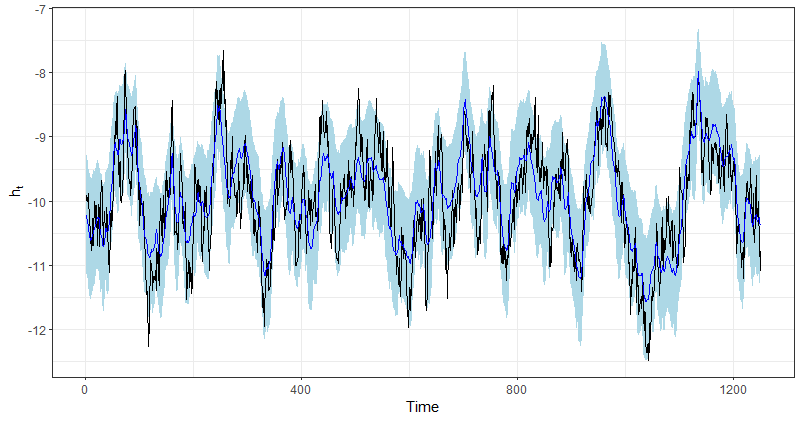
\includegraphics[width=340pt, height=200pt]{Chapters/chapter8/figures/SVmodel.png}
	\caption[List of figure caption goes here]{Stochastic volatility model.}\label{fig4}
\end{figure} 

So far, we have used MCMC algorithms to perform inference in \textit{state-space models}. These algorithms require all observations to estimate the unknown parameters, a process referred to as offline or batch inference. However, this approach has limitations when online inference is needed, as every new observation requires simulating a new posterior chain. This is because MCMC algorithms do not naturally adapt to sequential updates. In contrast, particle filter algorithms, which are a subset of sequential Monte Carlo (SMC) methods, are specifically designed for sequential use, making them suitable for online inference.    
     
Remember from Chapter \ref{chap5} that particle filters (sequential Monte Carlo) are algorithms that allow computing a numerical approximation to the filtering distribution $\pi(\bm{\theta}_{1:t}\mid \bm{y}_{1:t})$ sequentially in time. This is particularly relevant in non-linear and non-Gaussian models where there is no analytical solution for the filtering distribution.

The following code shows how to perform particle filtering in the vanilla stochastic volatility model assuming that the proposal distribution is the conditional prior distribution, that is, $q(h_t\mid h_{t-1},y_t)=\pi(h_t\mid h_{t-1})$, which is normal with mean $\mu+\phi(h_{t-1}-\mu)$ and variance $\sigma^2$. This choice implies that the incremental importance weights are equal to $p(y_t\mid h_t)$, which is $N(0,\exp(h_t))$. Therefore, the weights are proportional to the likelihood function. We perform multinomial resampling every time period in the code, and start the algorithm in the stationary distribution of $h_t$. Remember that there are other resampling approaches that are more efficient, for instance, residual resampling (see Section \ref{sec53}). We ask in Exercise 7 to modify this code to perform resampling when the effective sample size is lower than 50\% of the initial number of particles. In addition, we ask to program a sequential importance sampling, and check why is important to perform resampling in this simple example. 

Figure \ref{fig5} illustrates the filtering recursion using SMC with uneven weights (blue line), even weights (purple line), bands corresponding to plus/minus two standard deviations (light blue shaded area), and the true state (black line).\footnote{This standard deviation estimates the conditional posterior's standard deviation derived from the particles, not the estimator's standard deviation. The latter requires several independent particle runs on the same data.} The results indicate that SMC performs well even with a simple implementation, with no significant differences between using even and uneven weights (see Chapter \ref{chap5}).

In this example, we use the population parameters to perform the filtering recursion. However, this is not the case in practice, as we must estimate the time-invariant parameters. Therefore, more elaborate algorithms are required to achieve this (see Chapter \ref{chap5}). For instance, \cite{andrieu2010pmcmc} propose particle Markov chain Monte Carlo, a family of methods that combines MCMC and SMC. See \cite{dahlin2019getting} for a tutorial on particle Metropolis-Hastings in \textbf{R}. A potential practical solution for applications that require sequential updating of a posterior distribution over an unbounded time horizon is to estimate the time-invariant parameters offline using MCMC algorithms up to a specific time period, and then update the state vector sequentially online during subsequent time periods, iterating this process. This is not optimal, but it can be practical.

\begin{tcolorbox}[enhanced,width=4.67in,center upper,
	fontupper=\large\bfseries,drop shadow southwest,sharp corners]
	\textit{R code. Simulation and inference: Stochastic volatility model programming sequential Monte Carlo from scratch}
	\begin{VF}
		\begin{lstlisting}[language=R]
rm(list = ls()); set.seed(010101)
T <- 1250; mu <- -10; phi <- 0.95; sigma <- 0.3
h <- numeric(T); y <- numeric(T)
h[1] <- rnorm(1, mu, sigma / sqrt(1 - phi^2))  
y[1] <- rnorm(1, 0, exp(h[1] / 2))           
for (t in 2:T) {
	h[t] <- mu + phi*(h[t-1]-mu) + rnorm(1, 0, sigma)
	y[t] <- rnorm(1, 0, sd = exp(0.5*h[t]))
}
N <- 10000
log_Weights <- matrix(NA, N, T)  # Log weights
Weights <- matrix(NA, N, T)  # Weights 
WeightsST <- matrix(NA, N, T)  # Normalized weights 
WeightsSTT <- matrix(1/N, N, T)  # Normalized weights bar 
particles <- matrix(NA, N, T)   # Particles
particlesT <- matrix(NA, N, T)   # Particles bar
logalphas <- matrix(NA, N, T)   # Incremental importance 
particles[, 1] <- rnorm(N, mu, sigma / sqrt(1 - phi^2))  # Stationary prior
log_Weights[, 1] <- dnorm(y[1], 0, sd = exp(0.5*particles[,1]), log = TRUE)  # Likelihood
Weights[, 1] <- exp(log_Weights[, 1])
WeightsST[, 1] <- Weights[, 1] / sum(Weights[, 1])
ind <- sample(1:N, size = N, replace = TRUE, prob = WeightsST[, 1]) # Resample 
particles[, 1] <- particles[ind, 1] # Resampled particles
particlesT[, 1] <- particles[, 1] # Resampled particles
WeightsST[, 1] <- rep(1/N, N) # Resampled weights
pb <- txtProgressBar(min = 0, max = T, style = 3)
for (t in 2:T) {
	particles[, t] <- rnorm(N, mu + phi*(particles[, t - 1] - mu), sigma)  # Sample from proposal
	logalphas[, t] <- dnorm(y[t], 0, sd = exp(0.5*particles[,t]), log = TRUE) 
	Weights[, t] <- exp(logalphas[, t])
	WeightsST[, t] <- Weights[, t] / sum(Weights[, t])
	if(t < T){
		ind <- sample(1:N, size = N, replace = TRUE, prob = WeightsST[, t])
		particles[, 1:t] <- particles[ind, 1:t]
	}else{
		ind <- sample(1:N, size = N, replace = TRUE, prob = WeightsST[, t])
		particlesT[, 1:t] <- particles[ind, 1:t]
	}
	setTxtProgressBar(pb, t)
}
close(pb)
\end{lstlisting}
	\end{VF}
\end{tcolorbox}

\begin{tcolorbox}[enhanced,width=4.67in,center upper,
	fontupper=\large\bfseries,drop shadow southwest,sharp corners]
	\textit{R code. Simulation and inference: Stochastic volatility model programming sequential Monte Carlo from scratch}
	\begin{VF}
		\begin{lstlisting}[language=R]
FilterDist <- colSums(particles * WeightsST)
SDFilterDist <- (colSums(particles^2 * WeightsST) - FilterDist^2)^0.5
FilterDistT <- colSums(particlesT * WeightsSTT)
SDFilterDistT <- (colSums(particlesT^2 * WeightsSTT) - FilterDistT^2)^0.5
MargLik <- colMeans(Weights)
plot(MargLik, type = "l")
library(dplyr)
library(ggplot2)
require(latex2exp)
ggplot2::theme_set(theme_bw())
Tfig <- 250
keepFig <- 1:Tfig
df <- tibble(t = keepFig,
mean = FilterDist[keepFig],
lower = FilterDist[keepFig] - 2*SDFilterDist[keepFig],
upper = FilterDist[keepFig] + 2*SDFilterDist[keepFig],
meanT = FilterDistT[keepFig],
lowerT = FilterDistT[keepFig] - 2*SDFilterDistT[keepFig],
upperT = FilterDistT[keepFig] + 2*SDFilterDistT[keepFig],
x_true = h[keepFig])
plot_filtering_estimates <- function(df) {
	p <- ggplot(data = df, aes(x = t)) +
	geom_ribbon(aes(ymin = lower, ymax = upper), alpha = 1,
	fill = "lightblue") +
	geom_line(aes(y = x_true), colour = "black", alpha = 1,
	linewidth = 0.5) +
	geom_line(aes(y = mean), colour = "blue", linewidth = 0.5) +
	geom_line(aes(y = meanT), colour = "purple", linewidth = 0.5) +
	ylab(TeX("$h_{t}$")) + xlab("Time")
	print(p)
}
plot_filtering_estimates(df)
\end{lstlisting}
	\end{VF}
\end{tcolorbox} 

 
\begin{figure}[!h]
	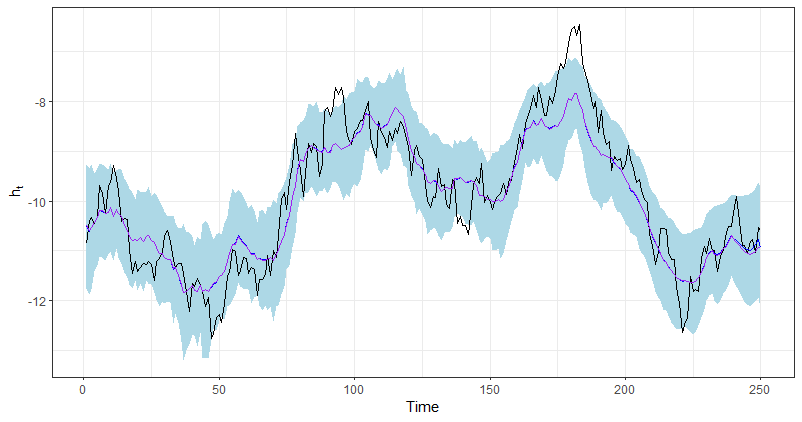
\includegraphics[width=340pt, height=200pt]{Chapters/chapter8/figures/SVSMC.png}
	\caption[List of figure caption goes here]{Stochastic volatility model: Sequential Monte Carlo (SMC).}\label{fig5}
\end{figure} 
  
\section{Vector Autoregressive models}\label{sec84}
Another widely used methodological approach in time series analysis is the vector autoregressive (VAR) model, which extends AR(p) models to the multivariate case. Since the seminal work by Sims (1980) \cite{sims1980macroeconomics}, these models have become a cornerstone of macroeconomic research to perform forecasts, and impulse-response (structural) analysis. This chapter provides an introduction to Bayesian inference in VAR models, with detailed discussions available in \cite{koop2010bayesian,DelNegro2011VAR,wozniak2016bayesian,chan2019bayesian}.

The \textit{reduced-form} VAR(p) model can be written as
\begin{align}\label{eqVAR}
	\bm{y}_t=\bm{v} + \sum_{j=1}^p\bm{A}_{j}\bm{y}_{t-j}+\bm{\mu}_t,
\end{align}
where $\bm{y}_t$ is a $M$-dimensional vector having information of $M$ time series variables, $\bm{v}$ is a $M$-dimensional vector of intercepts, $\bm{A}_{j}$ are $M\times M$ matrices of coefficients, and $\bm{\mu}_t \stackrel{iid}{\sim} N_M(\bm{0}, \bm{\Sigma})$ are stochastic errors, $t=1,2,\dots,T$ and $j=1,2,\dots,p$. Other deterministic terms and exogenous variables can be added to the specification without main difficulty, we do not do this to keep simply the notation. In addition, we assume that the stability condition is satisfied such that the stochastic process is stationary (see \cite[Chap.~2]{helmut2005new} for details), and we have available $p$ presample values for each variable. 

Following the matrix-form notation of the multivariate regression model (see sections \ref{sec44} and \ref{sec71}), we can set $\bm{Y}=\left[{\bm{y_{1}}} \ {\bm{y_{2}}} \ \ldots \ {\bm{y_{M}}}\right]$, which is an $ T\times M$ matrix, $\bm{x}_t=[1 \ \bm{y}_{t-1}^{\top} \ \dots \ \bm{y}_{t-p}^{\top}]$ is a $(1+Mp)$-dimensional row vector, we define $k=1+Mp$ to facilitate notation, and set \begin{align*}
\bm{X}=\begin{bmatrix}
	\bm{x}_1\\
	\bm{x}_2\\
	\vdots \\
	\bm{x}_T\\
\end{bmatrix},
\end{align*}
which is a $ T\times k$ matrix, $\bm{B}=\left[\bm{v} \ \bm{A}_{1} \ \bm{A}_{2} \ldots \bm{A}_{P}\right]^{\top}$ is a $ k \times M$ matrix of parameters, and $\bm{U}=\left[\bm{\mu}_{1} \ \bm{\mu}_{2}\ldots \bm{\mu}_{M}\right]$ is a $T\times M$-dimensional matrix of stochastic random errors such that $\bm{U}\sim N_{T\times M}(\bm{0}_{T\times M},\bm{\Sigma}\otimes \bm{I}_T)$. Thus, we can express the VAR(p) model in the form of a multivariate regression model,
\begin{align*}
	\bm{Y}=\bm{X}\bm{B}+\bm{U}.
\end{align*}
We can assume conjugate priors to facilitate computation, that is, 
\[
\pi({\bm{B}}, {\bm{\Sigma}}) = \pi({\bm{B}} \mid {\bm{\Sigma}}) \pi({\bm{\Sigma}}),
\]
where ${\bm{B}} \mid {\bm{\Sigma}} \sim N_{k \times M}({\bm{B}}_{0}, {\bm{V}}_{0}, {\bm{\Sigma}})$ and ${\bm{\Sigma}} \sim IW({\bm{\Psi}}_{0}, \alpha_{0})$. Thus, 
\[
\pi({\bm{B}}, {\bm{\Sigma}} \mid {\bm{Y}}, {\bm{X}}) = \pi({\bm{B}} \mid {\bm{\Sigma}}, {\bm{Y}}, {\bm{X}}) \pi({\bm{\Sigma}} \mid {\bm{Y}}, {\bm{X}}),
\]
where ${\bm{B}} \mid {\bm{\Sigma}}, {\bm{Y}}, {\bm{X}} \sim N_{k \times M}({\bm{B}}_n, {\bm{V}}_n, {\bm{\Sigma}})$ and ${\bm{\Sigma}} \mid {\bm{Y}}, {\bm{X}} \sim IW({\bm{\Psi}}_n, \alpha_n)$. The quantities ${\bm{B}}_n$, ${\bm{V}}_n$, ${\bm{\Psi}}_n$, and $\alpha_n$ are given by the following expressions:

\[
{\bm{B}}_n = ({\bm{V}}_{0}^{-1} + {\bm{X}}^{\top}{\bm{X}})^{-1}({\bm{V}}_{0}^{-1}{\bm{B}}_{0} + {\bm{X}}^{\top}{\bm{X}} \widehat{\bm{B}}),
\]
\[
{\bm{V}}_n = ({\bm{V}}_{0}^{-1} + {\bm{X}}^{\top}{\bm{X}})^{-1},
\]
\[
{\bm{\Psi}}_n = {\bm{\Psi}}_{0} + {\bm{S}} + {\bm{B}}_{0}^{\top}{\bm{V}}_{0}^{-1}{\bm{B}}_{0} + \widehat{\bm{B}}^{\top}{\bm{X}}^{\top}{\bm{X}} \widehat{\bm{B}} - {\bm{B}}_n^{\top} {\bm{V}}_n^{-1} {\bm{B}}_n,
\]
\[
{\bm{S}} = ({\bm{Y}} - {\bm{X}} \widehat{\bm{B}})^{\top}({\bm{Y}} - {\bm{X}} \widehat{\bm{B}}),
\]
\[
\widehat{\bm{B}} = ({\bm{X}}^{\top}{\bm{X}})^{-1}{\bm{X}}^{\top}{\bm{Y}},
\]
and 
\[
\alpha_n = T + \alpha_0.
\]

%We can assume conjugate priors to facilitate computation, that is, $\pi({\bm{B}},{\bm{\Sigma}})=\pi({\bm{B}}\mid {\bm{\Sigma}})\pi({\bm{\Sigma}})$ where ${\bm{B}}\mid {\bm \Sigma}\sim N_{k\times M}({\bm{B}}_{0},{\bm{V}}_{0},{\bm{\Sigma}})$ and ${\bm{\Sigma}}\sim IW({\bm{\Psi}}_{0},\alpha_{0})$. Thus, $\pi({\bm{B}},{\bm \Sigma}\mid  {\bm{Y}}, {\bm{X}})=\pi ({\bm{B}}\mid  {\bm \Sigma},{\bm{Y}},{\bm{X}})\pi({\bm \Sigma}\mid  {\bm{Y}},{\bm{X}})$ where ${\bm{B}}\mid  {\bm \Sigma},{\bm{Y}}, {\bm{X}} \sim N_{k\times M}({\bm{B}}_n,{\bm{V}}_n,{\bm \Sigma})$ and ${\bm \Sigma}\mid  {\bm{Y}},{\bm{X}} \sim IW({\bm{\Psi}}_n,{\alpha}_n)$, ${\bm{B}}_n = ({\bm{V}}_{0}^{-1}+{\bm{X}}^{\top}{\bm{X}})^{-1}({\bm{V}}_{0}^{-1}{\bm{B}}_{0}+{\bm{X}}^{\top}{\bm{X}}\widehat{\bm{B}})$, ${\bm{V}}_n = ({\bm{V}}_{0}^{-1}+{\bm{X}}^{\top}{\bm{X}})^{-1}$, ${\bm{\Psi}}_n={\bm{\Psi}}_{0}+{\bm{S}}+{\bm{B}}_{0}^{\top}{\bm{V}}_{0}^{-1}{\bm{B}}_{0}+\widehat{\bm{B}}^{\top}{\bm{X}}^{\top}{\bm{X}}\widehat{\bm{B}}-{\bm{B}}_n^{\top}{\bm{V}}_n^{-1}{\bm{B}}_n$, ${\bm{S}}= ({\bm{Y}}-{\bm{X}}\widehat{\bm{B}})^{\top}({\bm{Y}}-{\bm{X}}\widehat{\bm{B}})$, $\widehat{\bm{B}}= ({\bm{X}}^{\top}{\bm{X}})^{-1}{\bm{X}}^{\top}{\bm{Y}}$, and  $\alpha_n= T+\alpha_{0}$. 

Thus, we see that once we express a VAR(p) model in the correct form, we can perform Bayesian inference as we did in the multivariate regression model. However, assuming conjugate priors has some limitations. First, VAR(p) models have many parameters. For instance, with 4 lags and 6 variables, we would have 150 location parameters ($(1 + (6 \times 4)) \times 6$) and 21 scale parameters ($6 \times (6 + 1)/2$) for the covariance matrix. This can lead to a loss of precision, especially when using macroeconomic data, due to the typical lack of large sample sizes. Therefore, it is desirable to impose prior restrictions on the model specification, which cannot be achieved using conjugate priors. 

Second, natural conjugate priors do not allow for flexible extensions, such as having different regressors in different equations. Third, the prior structure implies that the prior covariance of the coefficients in any two equations must be proportional to each other. This is because the prior covariance form is $\bm{\Sigma} \otimes \bm{V}_0$. However, this does not always make sense in certain applications. For example, imposing zero prior restrictions on some coefficients would imply that the prior variance of these coefficients should be near zero, but this does not need to be true for all coefficients in the model.

To address the first issue, we can think of the VAR(p) specification in a similar way to the seemingly unrelated regression (SUR) model, where we have different regressors in different equations and account for unobserved dependence. This approach allows us to impose zero restrictions on the VAR(p) model, thereby improving its parsimony. Following the setup in Section \ref{sec72}, we have
\[
\bm{y}_{m} = \bm{Z}_{m} \bm{\beta}_m + \bm{\mu}_m,
\]
where $\bm{y}_m$ is a $T$-dimensional vector corresponding to the $m$-th time series variable, $\bm{Z}_m$ is a $T \times K_m$ matrix of regressors, $\bm{\beta}_m$ is a $K_m$-dimensional vector of location parameters, and $\bm{\mu}_m$ is a $T$-dimensional vector of stochastic errors, for $m = 1, 2, \dots, M$.

Stacking the $M$ equations, we can write $\bm{y}=\bm{Z}\bm{\beta}+\bm{\mu}$ where $\bm{y}=\left[\bm{y}_{1}^{\top} \ \bm{y}_{2}^{\top} \dots \bm{y}_{M}^{\top}\right]^{\top}$ is a $MT$-dimensional vector,  $\bm{\beta}=\left[\bm{\beta}_{1}^{\top} \ \bm{\beta}_{2}^{\top} \ldots \bm{\beta}_{M}^{\top}\right]^{\top}$ is a $ K$ dimensional vector, $K=\sum_{m=1}^{M} K_m$, note that having the same number of regressors implies $K = M \cdot k$ coefficients, $\bm{Z}$ is an $MT\times K$ block diagonal matrix composed of $\bm{Z}_{m}$, that is,
\begin{align*}
	\bm{Z}&=\begin{bmatrix}
		\bm{Z}_1 & \bm{0} & \dots & \bm{0}\\
		\bm{0} & \bm{Z}_2 & \dots & \bm{0}\\
		\vdots & \vdots & \ddots & \vdots\\
		\bm{0} & \bm{0} & \dots & \bm{Z}_M		
	\end{bmatrix},
\end{align*}
and $\bm{\mu}=\left[\bm{\mu}_{1}^{\top} \ \bm{\mu}_{2}^{\top} \dots \ \bm{\mu}_{M}^{\top}\right]^{\top}$ is a $MT$-dimensional vector of stochastic errors such that $\bm{\mu}\sim{N}(\bm{0},\bm{\Sigma}\otimes \bm{I}_T)$.

We can use independent priors in this model to overcome the limitations of the conjugate prior, that is, $\pi(\bm{\beta})\sim{N}(\bm{\beta}_0,\bm{B}_0)$ and $\pi(\bm{\Sigma}^{-1})\sim{W}(\alpha_0,\bm{\Psi}_0)$. Thus, we know from Section \ref{sec72} that the posterior distributions are
\begin{equation*}
	\bm{\beta}\mid \bm{\Sigma}, \bm{y}, \bm{Z} \sim {N}(\bm{\beta}_n, \bm{B}_n), 
\end{equation*}
\begin{equation*}
	\bm{\Sigma}^{-1}\mid \bm{\beta}, \bm{y}, \bm{Z} \sim {W}(\alpha_n, \bm{\Psi}_n),
\end{equation*}

where $\bm{B}_n=(\bm{Z}^{\top}(\bm{\Sigma}^{-1}\otimes \bm{I}_T )\bm{Z}+\bm{B}_0^{-1})^{-1}$, $\bm{\beta}_n=\bm{B}_n(\bm{B}_0^{-1}\bm{\beta}_0 + \bm{Z}^{\top}(\bm{\Sigma}^{-1}\otimes \bm{I}_T)\bm{y})$, $\alpha_n = \alpha_0 + T$ and $\bm{\Psi}_n = (\bm{\Psi}_0^{-1} + \bm{U}^{\top}\bm{U})^{-1}$, where $\bm{U}$ is an $T\times M$ matrix whose columns are $\bm{y}_m-\bm{Z}_m\bm{\beta}_m$.\footnote{We can also use the alternative representation presented in Section \ref{sec72}.}

Observe that we have standard conditional posteriors, thus, we can employ a Gibbs sampling algorithm to get the posterior draws. We can calculate the prediction $\bm{y}_{T+1}=[y_{1T+1} \ y_{2T+1} \ \dots \ y_{MT+1}]^{\top}$ knowing that $\bm{y}_{T+1}\sim N(\bm{Z}_{T}\bm{\beta},\bm{\Sigma})$, where \begin{align*}
	\bm{Z}_T&=\begin{bmatrix}
		\bm{z}_{1T}^{\top} & 0 & \dots & 0\\
		0 & \bm{z}_{2T}^{\top} & \dots & 0\\
		\vdots & \vdots & \ddots & \vdots\\
		0 & 0& \dots & \bm{z}_{MT}^{\top}		
	\end{bmatrix},
\end{align*} 
and using the posterior draws of $\bm{\beta}^{(s)}$ and $\bm{\Sigma}^{(s)}$, $s=1,2,\dots,S$. We can also perform inference of functions of the parameters that are of main interest when using VAR models.

Note that independent priors offer more flexibility regarding prior information. For instance, we can set $\bm{\Psi}_0 = \bm{S}^{-1}$, $\alpha_0 = T$, $\bm{\beta}_0 = \bm{0}$, and $\bm{B}_0$ as a diagonal matrix, where the variance of the components associated with the coefficients in the $m$-th equation is such that the prior variance of the coefficients for the own lags is $a_1/l^2$, the variances for lag $l$ of variable $m \neq j$ are $a_2s_{m}^2/(l^2 s_{j}^2)$, and the variance of the intercepts is set to $a_3 s_{m}^2$, with $l = 1, 2, \dots, p$, where $s_m$ is the estimated standard error of the residuals from an unrestricted univariate autoregression of variable $m$ against a constant and its $p$ lags \cite{litterman1986forecasting, koop2010bayesian}. 

Note that setting $a_1 > a_2$ implies that own lags are more important as predictors than lags of other variables, and dividing by $l^2$ implies that more recent lags are more relevant than those further in the past. The specific choices of $a_1$, $a_2$, and $a_3$ ($a_k > 0$, $k = 1, 2, 3$) depend on the specific application, but it is generally easier to elicit these parameters rather than the $K(K+1)/2$ different components of $\bm{B}_0$.\footnote{In our GUI, we use the \textit{bvartools} package, which adopts a slightly different notation such that $a_2 = a_1 \kappa_2$ and $a_3 = a_1 \kappa_3$. Thus, we need to set $a_1$, $\kappa_2$, and $\kappa_3$.}

This setting is known as the \textit{Minnesota prior}, as it is based on the seminal proposals for Bayesian VAR models by researchers at the University of Minnesota and the Federal Reserve Bank of Minneapolis \cite{doan1984forecasting, litterman1986forecasting}.\footnote{In the case that the variables are not stationary, which is more likely when using variables in levels (e.g., gross domestic product), we set $\bm{\beta}_0 = \bm{0}$, except for the elements associated with the first own lags of the dependent variables in each equation, where the prior mean is set to 1. Additionally, the original proposal of the Minnesota prior set $\bm{\Sigma} = \bm{S}/T$, meaning it did not account for uncertainty regarding $\bm{\Sigma}$.}

An important non-linear function of parameters when performing VAR analysis is the \textit{impulse response} function, which is, the response of one variable to an impulse in another variable in the model. The \textit{impulse response} function can be deduced using the $MA$ representation of the VAR model. In particular, we can write Equation \ref{eqVAR} using the lag operator (see Section \ref{sec82}),
\begin{align}\label{eqVAR1}
	\bm{y}_t=\bm{v} + (\bm{A}_{1}L+\bm{A}_{2}L^2+\dots+\bm{A}_{p}L^p)\bm{y}_t+\bm{\mu}_t,
\end{align}
thus $\bm{A}(L)\bm{y}_t=\bm{v}+\bm{\mu}_t$, where $\bm{A}(L)=\bm{I}_M-\bm{A}_{1}L-\bm{A}_{2}L^2-\dots-\bm{A}_{p}L^p$. Let $\bm{\Phi}(L):= \sum_{s=0}^{\infty}\bm{\Phi}_sL^s$ an operator such that $\bm{\Phi}(L)\bm{A}(L)=\bm{I}_M$. Thus, we have that  $\bm{\Phi}(L)\bm{A}(L)\bm{y}_t=\left(\sum_{s=0}^{\infty}\bm{\Phi}_sL^s\right)\bm{v}+\left(\sum_{s=0}^{\infty}\bm{\Phi}_sL^s\right)\bm{\mu}_{t}=\bm{\mu}+\sum_{s=0}^{\infty}\bm{\Phi}_s\bm{\mu}_{t-s}$. Note that $L^s\bm{v}=\bm{v}$ because $\bm{v}$ is constant, thus we set $\sum_{s=0}^{\infty}\bm{\Phi}_sL^s\bm{v}=\sum_{s=0}^{\infty}\bm{\Phi}_s\bm{v}=\bm{\Phi}(1)\bm{v}=(\bm{I}_M-\bm{A}_{1}-\bm{A}_{2}-\dots-\bm{A}_{p})^{-1}\bm{v}:=\bm{\mu}$, which is the mean of the process \cite[Chap.~2]{helmut2005new}. Therefore, the MA representation of the VAR is
\begin{align}\label{eqMA}
	\bm{y}_t=\bm{\mu} + \sum_{s=0}^{\infty}\bm{\Phi}_s\bm{\mu}_{t-s},
\end{align}
where $\bm{\Phi}_0=\bm{I}_M$, and we can get the coefficients in $\bm{\Phi}_s$ by the recursion $\bm{\Phi}_s=\sum_{l=1}^s\bm{\Phi}_{s-l}\bm{A}_l$, $\bm{A}_l=\bm{0}$, $l>p$ and $s=1,2,..$ \cite[Chap.~2]{helmut2005new}. This impulse response function is called \textit{forecast error impulse response function}.

The MA coefficients contain the impulse responses of the system. In particular, $\phi_{mj,s}$, which is the $mj$-th element of the matrix $\bm{\Phi}_s$, represents the response of the $m$-th variable to a unit shock of the variable $j$ in the system, $s$ periods ago, provided that the effect is not contaminated by other shocks in the system. The long-term effects (total multipliers) are given by $\bm{\Psi}_{\infty}:=\sum_{s=1}^{\infty}\bm{\Phi}_s=(\bm{I}_M-\bm{A}_{1}-\bm{A}_{2}-\dots-\bm{A}_{p})^{-1}$.

An assumption in these \textit{impulse response} functions is that a shock occurs in only one variable at a time. This can be questionable as different shocks may be correlated, consequently, occurring simultaneously. Thus, the \textit{impulse response} analysis can be performed based on the alternative MA representation, $\bm{y}_t=\bm{\mu} + \sum_{s=0}^{\infty}\bm{\Phi}_s\bm{P}\bm{P}^{-1}\bm{\mu}_{t-s}=\bm{\mu} + \sum_{s=0}^{\infty}\bm{\Theta}_s\bm{w}_{t-s}$, where $\bm{\Theta}_s=\bm{\Phi}_s\bm{P}$ and $\bm{w}_{t}=\bm{P}^{-1}\bm{\mu}_{t}$, $\bm{P}$ is a lower triangular matrix such that $\bm{\Sigma}=\bm{P}\bm{P}^{\top}$ (Cholesky factorization/decomposition). Note that the covariance matrix of $\bm{w}_t$ is $\bm{I}_M$ due to $\mathbb{E}[\bm{w}_t\bm{w}_t^{\top}]=\mathbb{E}[\bm{P}^{-1}\bm{\mu}_{t}\bm{\mu}_t^{\top}(\bm{P}^{-1})^{\top}]=\bm{P}^{-1}\bm{\Sigma}(\bm{P}^{-1})^{\top}=\bm{P}^{-1}\bm{P}\bm{P}^{\top}(\bm{P}^{-1})^{\top}=\bm{I}_M$. 

In this representation is sensible to assume that each shock occurs independently due to the covariance matrix of $\bm{w}_t$ being an identity. In addition, a unit shock is a shock of size one standard deviation due the result of the covariance matrix. This is named the \textit{ortogonalized impulse response}, where $\theta_{mj,s}$, which is the $mj$-th element of the matrix $\bm{\Theta}_s$, represents the response of the $m$-th variable to a standard deviation shock of the variable $j$ in the system, $s$ periods ago. The critical point with the ortogonalized impulse responses is that the order of the variables in the VAR is really important because implicitly establishes a recursive model, that is, the $m$-th equation in the system may contain $y_{1t}, y_{2t}, \dots, y_{m-1t}$, but not $y_{mt}, y_{m+1t}, \dots, y_{Mt}$ on the hand-right side of its equation. Thus, $y_{mt}$ cannot have an instantaneous impact on $y_{jt}$ for $j<m$ \cite[Chap.~2]{helmut2005new}.

Beyond the fascinating macroeconomic implications embedded in the specification of VAR models, the key point for this section is that we can infer impulse response functions using the posterior draws.\\

\textbf{Example: US fiscal system}

Let's use the dataset provided by \cite{Tomasz2024} of the US fiscal system, where \textit{ttr} is the quarterly total tax revenue, \textit{gs} is the quarterly total government spending, and \textit{gdp} is the quarterly gross domestic product, all expressed in log, real, per person terms, and the period is 1948q1 to 2024q2. This dataset is the \textit{18USAfiscal.csv} file. \cite{mertens2014reconciliation} analyze the US fiscal policy shocks using these variables.

Let's estimate a VAR model where $\bm{y}_t=[\Delta(ttr_t) \ \Delta(gs_t) \ \Delta(gdp_t)]^{\top}$, that is, we work with the log differences (variation rates), and we set $p=1$. We use the package \textit{bvartools} to estimate the \textit{forecast error} and \textit{ortogonalized} impulse response functions. We use vague independent priors setting $\bm{\beta}_0=\bm{0}$, $\bm{B}_0=100\bm{I}$, $\bm{V}_0=5^{-1}\bm{I}$ and $\alpha_0=3$, and the Minnesota prior setting $a_1=2$, $\kappa_2=0.5$ and $\kappa_3=5$ (default values).\footnote{The \textit{bvartools} package uses the inverse Wishart distribution as prior for $\bm{\Sigma}$, where the hyperparameters are the degrees of freedom of the error term, and the prior error variance of endogenous variables.}

The following code shows how to do this, take into account that we use the first 301 observations to estimate the model, and keep the last 4 observations to check the forecasting performance. Figures \ref{fig6} and \ref{fig7} show the impulse response functions of \textit{gs} with respect to \textit{gs}, the \textit{forecast error impulse response} using vague independent priors, and the \textit{orthogonalized impulse response} using the Minnesota prior, respectively. We see that the effect of the Minnesota prior is to decrease uncertainty. In addition, the forecasting exercise results indicate that these assumptions have same effects in this example. In particular, Figure \ref{fig8} shows that the mean forecasts using the vague prior (green line) and the Minnesota prior (red line) are indistinguishable from the true observations (black line). However, the Minnesota prior enhances forecast precision, as its 95\% predictive interval (blue shaded area) is narrower and fully contained within the 95\% predictive interval obtained using vague priors (light blue shaded area). This improvement is attributable to the shrinkage properties of the Minnesota prior.

\begin{tcolorbox}[enhanced,width=4.67in,center upper,
	fontupper=\large\bfseries,drop shadow southwest,sharp corners]
	\textit{R code. VAR model: US fiscal shocks}
	\begin{VF}
		\begin{lstlisting}[language=R]
rm(list = ls()); set.seed(010101)
DataUSfilcal <- read.csv("https://raw.githubusercontent.com/besmarter/BSTApp/refs/heads/master/DataApp/18USAfiscal.csv", sep = ",", header = TRUE, quote = "")
attach(DataUSfilcal) # upload data
Y <- cbind(diff(as.matrix(DataUSfilcal[,-c(1:2)])))
T <- dim(Y)[1]-1; K <- dim(Y)[2]
Ynew <- Y[-c((T-2):(T+1)), ] # Use 4 last observations to check forecast
y1 <- Ynew[-1, 1]; y2 <- Ynew[-1, 2]; y3 <- Ynew[-1, 3]
X1 <- cbind(1, lag(Ynew)); X1 <- X1[-1,]
X2 <- cbind(1, lag(Ynew)); X2 <- X2[-1,]
X3 <- cbind(1, lag(Ynew)); X3 <- X3[-1,]
M <- dim(Y)[2]; K1 <- dim(X1)[2]; K2 <- dim(X2)[2]; K3 <- dim(X3)[2] 
K <- K1 + K2 + K3
# Hyperparameters
b0 <- 0; c0 <- 100; V0 <- 5^(-1); a0 <- M
#Posterior draws
MCMC <- 10000; burnin <- 1000; H <- 10; YnewPack <- ts(Ynew)
model <- bvartools::gen_var(YnewPack, p = 1, deterministic = "const", iterations = MCMC, burnin = burnin) # Create model
model <- bvartools::add_priors(model, coef = list(v_i = c0^-1, v_i_det = c0^-1, const = b0), sigma = list(df = a0, scale = V0/a0), coint_var = FALSE) # Add priors
object <- bvartools::draw_posterior(model) # Posterior draws
ir <- bvartools::irf.bvar(object, impulse = "gs", response = "gs", n.ahead = H, type = "feir", cumulative = FALSE) # Calculate IR
# Plot IR
plot_IR <- function(df) {
	p <- ggplot(data = df, aes(x = t)) + geom_ribbon(aes(ymin = lower, ymax = upper), alpha = 1, fill = "lightblue") + geom_line(aes(y = mean), colour = "blue", linewidth = 0.5) + ylab("Impulse response") + xlab("Time") + xlim(0,H)
	print(p)
}
dfNew <- tibble(t = 0:H, mean = as.numeric(ir[,2]), lower = as.numeric(ir[,1]), upper = as.numeric(ir[,3]))
FigNew <- plot_IR(dfNew)
# Using Minnesota prior
library(tibble)
modelMin <- bvartools::gen_var(YnewPack, p = 1, deterministic = "const", iterations = MCMC, burnin = burnin)
modelMin <- bvartools::add_priors(modelMin, minnesota = list(kappa0 = 2, kappa1 = 0.5, kappa3 = 5), coint_var = FALSE) # Minnesota prior
objectMin <- bvartools::draw_posterior(modelMin) # Posterior draws
irMin <- bvartools::irf.bvar(objectMin, impulse = "gs", response = "gs", n.ahead = H, type = "feir", cumulative = FALSE) # Calculate IR
dfNewMin <- tibble(t = 0:H, mean = as.numeric(irMin[,2]), lower = as.numeric(irMin[,1]), upper = as.numeric(irMin[,3]))
FigNewMin <- plot_IR(dfNewMin)
\end{lstlisting}
	\end{VF}
\end{tcolorbox} 

\begin{tcolorbox}[enhanced,width=4.67in,center upper,
	fontupper=\large\bfseries,drop shadow southwest,sharp corners]
	\textit{R code. VAR model: US fiscal shocks}
	\begin{VF}
		\begin{lstlisting}[language=R]
### Forecasting
bvar_pred <- predict(object, n.ahead = 4, new_d = rep(1, 4))
bvar_predOR <- predict(objectMin, n.ahead = 4, new_d = rep(1, 4))
dfFore <- tibble(t = c((T-2):(T+1)), mean = as.numeric(bvar_pred[["fcst"]][["gs"]][,2]), lower = as.numeric(bvar_pred[["fcst"]][["gs"]][,1]), upper = as.numeric(bvar_pred[["fcst"]][["gs"]][,3]), mean1 = as.numeric(bvar_predOR[["fcst"]][["gs"]][,2]), lower1 = as.numeric(bvar_predOR[["fcst"]][["gs"]][,1]), upper1 = as.numeric(bvar_predOR[["fcst"]][["gs"]][,3]), true = as.numeric(Y[c((T-2):(T+1)),2]))
plot_FORE <- function(df) {
	p <- ggplot(data = dfFore, aes(x = t)) + geom_ribbon(aes(ymin = lower1, ymax = upper1), alpha = 1, fill = "blue") + geom_ribbon(aes(ymin = lower, ymax = upper), alpha = 1, fill = "lightblue") + geom_line(aes(y = mean), colour = "green", linewidth = 0.5) + geom_line(aes(y = mean1), colour = "red", linewidth = 0.5) + geom_line(aes(y = true), colour = "black", linewidth = 0.5) + ylab("Forecast") + xlab("Time") + xlim(c((T-2),(T+1)))
	print(p)
}
FigFore <- plot_FORE(dfFore)
\end{lstlisting}
	\end{VF}
\end{tcolorbox} 


\begin{figure}[!h]
	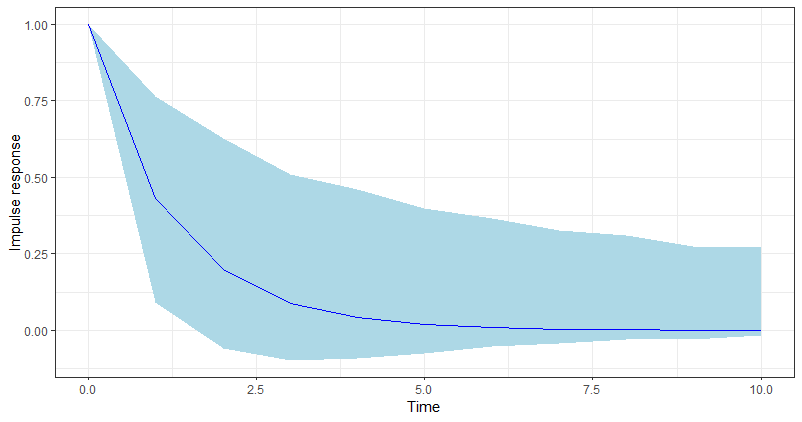
\includegraphics[width=340pt, height=200pt]{Chapters/chapter8/figures/IRsgsgFE.png}
	\caption[List of figure caption goes here]{Forecasting error impulse response: the government spending (\textit{gs}) with respect to the government spending (\textit{gs}).}\label{fig6}
\end{figure}

\begin{figure}[!h]
	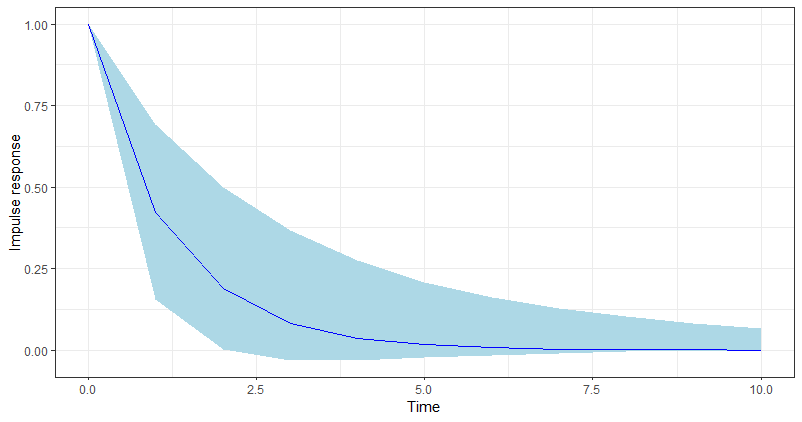
\includegraphics[width=340pt, height=200pt]{Chapters/chapter8/figures/IRsgsgO.png}
	\caption[List of figure caption goes here]{Ortogonalized impulse response: the government spending (\textit{gs}) with respect to the government spending (\textit{gs}).}\label{fig7}
\end{figure}

\begin{figure}[!h]
	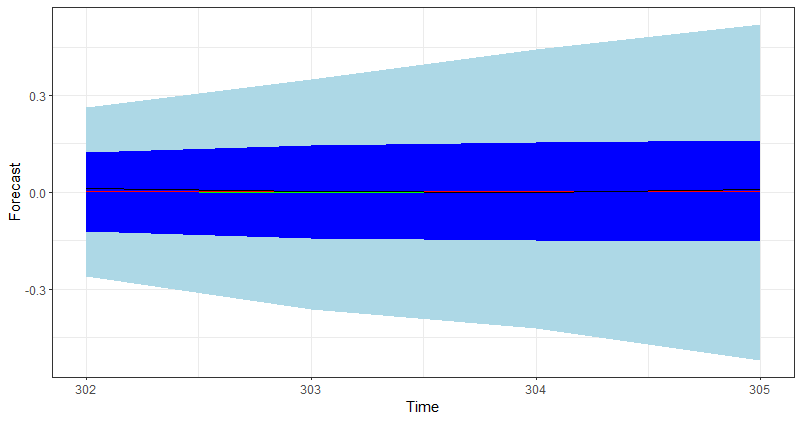
\includegraphics[width=340pt, height=200pt]{Chapters/chapter8/figures/Forecastgs.png}
	\caption[List of figure caption goes here]{Forecast performance: the government spending (\textit{gs}).}\label{fig8}
\end{figure}

Algorithm \ref{alg:VAR} shows how to do perform inference in VAR models using our GUI. See also Chapter \ref{chapGUI} for details regarding the dataset structure. 

\begin{algorithm}[h!]
	\caption{Vector Autoregressive models}\label{alg:VAR}
	\begin{algorithmic}[1]  		 			
		\State Select \textit{Time series Model} on the top panel
		\State Select \textit{VAR models} using the left radio button
		\State Upload the dataset selecting first if there is header in the file, and the kind of separator in the \textit{csv} file of the dataset (comma, semicolon, or tab). Then, use the \textit{Browse} button under the \textbf{Choose File} legend
		\State Select MCMC iterations, burn-in and thinning parameters using the \textit{Range sliders}
		\State Set the number of lags ($p$)
		\State Set the hyperparameters for the Minnesota prior: $a_1$, $\kappa_2$ and $\kappa_3$. This step is not necessary as by default our GUI uses default values in \textit{bvartools} package
		\State Select the type of \textit{impulse response functions}: forecast error or orthogonalized, and ordinary or cumulative.
		\State Set the time horizon for the impulse response functions and the forecasts 
		\State Click the \textit{Go!} button
		\State Analyze results
		\State Download impulse responses and forecasts using the \textit{Download Results} button
	\end{algorithmic} 
\end{algorithm}

There are other good packages in \textbf{R} to perform Bayesian inference in VAR models. For instance, \textit{bayesianVARs} package implements inference of reduced-form VARs with stochastic volatility \cite{Gruber2024}, \textit{BVAR} package performs inference using hierarchical priors \cite{Kuschnig2024}, \textit{bvarsv} implements time-varying parameters models \cite{Krueger2022}, \textit{bsvars} performs estimation of structural VAR models \cite{Tomasz2024}, and \textit{bsvarSIGNs} to estimating structural VAR models with sign restrictions \cite{Wang2024}. 
 
\section{Summary}\label{sec85}
We present a brief review of Bayesian inference in time series models. In particular, we introduce the \textit{state-space} representation and demonstrate how to perform inferential analysis for these models, focusing on the dynamic linear model and the stochastic volatility model. Additionally, we show how $ARMA(p,q)$ processes can be expressed in \textit{state-space} form and provide methods for estimating such models.

We also include code for implementing computational inference algorithms, such as sequential Monte Carlo (SMC), Hamiltonian Monte Carlo (HMC), and various Markov chain Monte Carlo (MCMC) methods. Finally, we introduce VAR(p) models, detailing how to perform impulse-response analysis and forecasting within this framework.

Time series analysis is a highly active research area with remarkable methodological developments and applications. Interested readers can refer to excellent materials in chapters 7 and 9 of \cite{geweke2011oxford}, and chapters 17 to 20 of \cite{chan2019bayesian}, along with the references therein.

\section{Exercises}\label{sec86}

\begin{enumerate}
	\item Simulate the \textit{dynamic linear model} assuming $X_t\sim N(1, 0.1\sigma^2)$, $w_t\sim N(0, 0.5\sigma^2)$, $\mu_t\sim N(0, \sigma^2)$, $\beta_0=1$, ${B}_0=0.5\sigma^2$, $\sigma^2=0.25$, and ${G}_t=1$, $t=1,\dots,100$. Then, perform the filtering recursion fixing $\Sigma=25\times 0.25$, $\Omega_1=0.5\Sigma$ (high signal-to-noise ratio) and  $\Omega_2=0.1\Sigma$ (low signal-to-noise ratio). Plot and compare the results. 	
	
	\item Simulate the \textit{dynamic linear model} $y_t=\beta_t x_t + \mu_t$, $\beta_t=\beta_{t-1}+w_t$, where $x_t\sim N(1, 0.1\sigma^2)$, $w_t\sim N(0, 0.5\sigma^2)$, $\mu_t\sim N(0, \sigma^2)$, $\beta_0=0$, $B_0=0.5\sigma^2$, and $\sigma^2=1$, $t=1,\dots,100$. Perform the filtering and smoothing recursions from scratch. 	
	
	\item Simulate the process $y_t=\alpha z_t + \beta_t x_t + \bm{h}^{\top}\bm{\epsilon}_t$, $\beta_t=\beta_{t-1}+\bm{H}^{\top}\bm{\epsilon}_t$, where $\bm{h}^{\top}=[1 \ 0]$, $\bm{H}^{\top}=[0 \ 1/\tau]$, $\bm{v}_t\sim N(\bm{0}_2, \sigma^2\bm{I}_2)$, $x_t\sim N(1, 2\sigma^2)$, $z_t\sim N(0, 2\sigma^2)$, $\alpha=2$, $\tau^2=5$ and $\sigma^2=0.1$, $t=1,\dots,200$. Assume $\pi({\beta}_0,{\alpha},\sigma^2,{\tau})=\pi({\beta}_0)\pi({\alpha})\pi(\sigma^2)\pi(\tau^2)$ where $\sigma^2\sim IG(\alpha_0/2,\delta_0/2)$, $\tau^2\sim G(v_{0}/2,v_{0}/2)$, ${\alpha}\sim N({a}_0,{A}_0)$ and ${\beta}_0\sim N({b}_0,{B}_0)$ such that $\alpha_0=\delta_0=1$, $v_0=5$, $a_0=0$, $A_0=1$, $\beta_0=0$, $B_0=\sigma^2/\tau^2$. Program the MCMC algorithm including the \textit{simulation smoother}.
	
	\item Show that the posterior distribution of $\bm{\phi}\mid \bm{\beta},\sigma^2,\bm{y},\bm{X}$ in the model $y_t=\bm{x}_t^{\top}\bm{\beta}+\mu_t$ where $\phi(L)\mu_t=\epsilon_t$ and $\epsilon_t\stackrel{iid}{\sim}N(0,\sigma^2)$ is $N(\bm{\phi}_n, \bm{\Phi}_n)\mathbbm{1}(\bm{\phi}\in S_{\bm{\phi}})$, where $\bm{\Phi}_n=(\bm{\Phi}_0^{-1}+\sigma^{-2}\bm{U}^{\top}\bm{U})$, $\bm{\phi}_n=\bm{\Phi}_n(\bm{\Phi}_0^{-1}\bm{\phi}_0+\sigma^{-2}\bm{U}^{\top}\bm{\mu})$, and $S_{\phi}$ is the stationary region of $\bm{\phi}$.	  
	
	\item Show that in the $AR(2)$ stationary process, $y_t=\mu+\phi_1y_{t-1}+\phi_2y_{t-2}+\epsilon_t$, where $\epsilon_t\sim N(0,\sigma^2)$, $\mathbb{E}[y_t]=\frac{\mu}{1-\phi_1-\phi_2}$, and $Var[y_t]=\frac{\sigma^2(1-\phi_2)}{1-\phi_2-\phi_1^2-\phi_1^2\phi_2-\phi_2^2+\phi_2^3}$.
	
	\item Program a Hamiltonian Monte Carlo taking into account the stationary restrictions on $\phi_1$ and $\phi_2$, and $\epsilon_0$ such that the acceptance rate is near 65\%. 
	
	\item \textbf{Stochastic volatility model}
	\begin{itemize}
		\item Program a sequential importance sampling (SIS) from scratch in the vanilla stochastic volatility model setting $\mu=-10$, $\phi = 0.95$, $\sigma=0.3$ and $T=250$. Check what happen with its performance.
		\item Modify the sequential Monte Carlo (SMC) to perform multinomial resampling when the effective sample size is lower than 50\% the initial number of particles.  
	\end{itemize}

	\item Estimate the vanilla stochastic volatility model using the dataset \textit{17ExcRate.csv}, provided by \cite{ramirez2024testing}, which contains the exchange rate log daily returns for USD/EUR, USD/GBP, and GBP/EUR from one year before and after the WHO declared the COVID-19 pandemic on 11 March 2020.
		
	\item Simulate the VAR(1) process
	\begin{align*}
		\begin{bmatrix}
			y_{1t}\\
			y_{2t}\\
			y_{3t}\\
		\end{bmatrix} = \begin{bmatrix}
			2.8\\
			2.2\\
			1.3\\
		\end{bmatrix} + \begin{bmatrix}
			0.5 & 0 & 0\\
			0.1 & 0.1 & 0.3\\
			0 & 0.2 & 0.3\\
		\end{bmatrix} \begin{bmatrix}
			y_{1t-1}\\
			y_{2t-1}\\
			y_{3t-1}\\
		\end{bmatrix} +\begin{bmatrix}
			\mu_{1t}\\
			\mu_{2t}\\
			\mu_{3t}\\
		\end{bmatrix},
	\end{align*}
	where $\bm{\Sigma}= \begin{bmatrix}
		2.25 & 0 & 0\\
		0 & 1 & 0.5\\
		0 & 0.5 & 0.74\\
	\end{bmatrix}$.

\begin{itemize}
	\item  Use vague independent priors setting $\bm{\beta}_0=\bm{0}$, $\bm{B}_0=100\bm{I}$, $\bm{V}_0=5\bm{I}$ and $\alpha_0=3$, and estimate a VAR(1) model using the \textit{rsurGibbs} function from the package \textit{bayesm}. Then, program from scratch algorithms to perform inference of the \textit{forecast error} and \textit{ortogonalized} impulse response functions, and compare with the population impulse response functions, that is, using the population parameters.
	
	\item Using the previous setting perform inference of the \textit{forecast error} and the \textit{ortogonalized} impulse responses using the package \textit{bvartools}.  
\end{itemize}

	
	
\end{enumerate}
